\documentclass[12pt]{article} % Change the float specifier from `h` to `ht`
\usepackage{graphicx} % Required for inserting images
\usepackage{blindtext}
\usepackage{titlesec}
\usepackage[italian]{babel}
\usepackage{relsize}
\usepackage{fancyhdr}
\usepackage[left=3cm,right=3cm, margin=3cm, vmargin=3cm]{geometry} % Imposta i margini laterali a 3 cm
\renewcommand{\familydefault}{\sfdefault}
\usepackage{subcaption} % pacchetto per le subfigure
\usepackage{listings}
\lstset{
language={[x86masm]Assembler}, % Imposta il linguaggio del codice
basicstyle=\ttfamily\footnotesize, % Stile di base con dimensione del font ridotta
tabsize=4, % Dimensione delle tabulazioni
showstringspaces=false, % Non mostrare spazi nelle stringhe
numbers=left, % Posizione dei numeri di riga
numberstyle=\tiny, % Stile dei numeri di riga
breaklines=true, % Permette la suddivisione automatica delle righe lunghe
frame=single % Aggiunge un bordo intorno al codice
}

\title{\Huge{Architettura degli Elaboratori}}
\author{\large{Alessia Cassetta}}
\date{Marzo 2024}

\begin{document}
\maketitle
\newpage
\tableofcontents
\newpage
\section{Storia} \subsection{Calcolo manuale} Gli antropologi fanno risalire alla fibula di babbuino ritrovato in una grotta abitata durante il Paleolitico [2.5 milioni a.C. a 10000 a.C.] sui monti Lebombo (Sudafrica) il primo datario. La presenza delle 29 incisioni suggerisce che potrebbe essere stato usato come un contatore di fasi lunari.
\par\medskip\noindent
\textbf{Alfabeto numerico}, insieme di simboli utili per rappresentare grandi quantità di beni, altrimenti non descrivibili. La \textbf{tavoletta di argilla} è il primo dispositivo utilizzato per rappresentare e archiviare delle quantità numeriche nonché per svolgere i calcoli in maniera manuale.
Abaco primo dispositivo per rappresentare e manipolare operandi mediante un particolare sistema posizionale in cui dei sassolini (calcolus) indicavano le unità, le decine e le centinaia in accordo alla loro presenza su delle linee pre-segnate. \par\medskip\noindent
La macchina di \textbf{Antikythera} è il \textbf{più antico calcolatore meccanico conosciuto}.  Si trattava di un sofisticato planetario, mosso da ruote dentate, che serviva per calcolare il sorgere del sole, le fasi lunari, i movimenti dei cinque pianeti allora conosciuti, gli equinozi, i mesi, i giorni della settimana e le date dei giochi olimpici.
Nel 1202, con il Liber Abaci, scritto da Leonardo Fibonacci matematico pisano, si introduce ufficialmente in Europa il \textbf{sistema posizionale}.
\par\medskip\noindent
Un primo sistema di calcolo (temporale) meccanico si riscontrò tra il 1230 ed il 1270 con l'orologio. Era un dispositivo costituito da un organo motore (es.: un peso o una molla); degli ingranaggi a ruote dentate che demoltiplicavano il moto, un elemento di distribuzione di un intervallo di tempo (lo scappamento) regolato da un componente con moto isocrono (es.: un pendolo) e un indicatore della misurazione il quadrante).
\par\medskip\noindent
\subsection{Il Calcolo Semi-AUtomatico}
Nel 1623 il matematico tedesco Wilhelm Schickard progetta e realizza un prototipo di \textbf{prima macchina calcolatrice meccanica}, il Calculating Clock.\par\medskip\noindent
Nel 1642 il matematico e filosofo francese Blaise Pascal propose il \textbf{Pascaline}, una macchina automatica in grado di svolgere l’operazione di addizione e di sottrazione.
\par\medskip\noindent
Nel 1672 il filosofo e matematico Gottfried Wilhelm Leibniz, famoso per lo studio aritmetico del sistema binario, perfezionò il Pascaline con il \textbf{Contatore a gradini} (calcolatrice a pignoni o Leibniz Machine). Si trattava di una macchina di calcolo manuale in grado di svolgere le quattro operazioni elementari (somma, sottrazione, moltiplicazione e divisione). Migliorato nel 1727 da Jacob Leupold e, più avanti, dal francese Thomas de Colmar con l’invenzione dell’aritmometro.
\par\medskip\noindent
Nel 1816 Charles Babbage, richiamando le tecniche di semi automazione dei telai meccanici di Joseph Jacquard, progetta la\textbf{ macchina differenziale}. La Difference Engine era una calcolatrice, la cui meccanica era attivata da un motore a vapore. Oltre alle normali operazioni aritmetiche, era in grado di svolgere il calcolo polinomiale (per la risoluzione di funzioni logaritmiche, serie di Taylor).
\subsection{Macchine Programmate}
Il prototipo di una macchina programmata automatica deputata al calcolo fu proposto nel 1890 da Herman Hollerith per il censimento dei cittadini statunitensi: Hollerith Tabulator o Tabulator Machine.
\par\medskip\noindent
L’invenzione faceva uso di schede cartacee perforabili (punch cards) su cui erano impresse, in posizioni prestabilite, le caratteristiche demografiche (stato civile, luogo di nascita, età, Stato di residenza).\par\medskip\noindent
Le macchine programmate proposte da Hollerith, però, avevano il limite di non poter discriminare, o contare, più caratteristiche demografiche allo stesso momento. Per individuare tutte le donne residenti a Boston bisognava dapprima selezionare le tessere con foratura sul campo F e poi compiere una nuova cernita considerando la colonna indicante la città di residenza Boston. Nei modelli successivi Hollerith introdusse i \textbf{pannelli programmati} grazie ai quali si consentì la selezione di schede aventi più caratteristiche demografiche durante la stessa analisi. I pannelli programmati erano dotati di fili interconnessi con dei componenti attivi che simulavano gli operatori logici (and e or) dell’Algebra di Boole. I pannelli erano sostituibili e la disposizione dei cavi e degli interruttori logici fu data in incarico a una nuova figura professionale: \textbf{il programmatore}\par\medskip\noindent
Nel 1889, Dorr Eugene Felt realizzò Comptometer, \textbf{una calcolatrice dotata di tastiera che riproduceva il risultato su un nastro cartaceo}. Il primo esemplare fu realizzato con una scatola per la pasta, tanto da prendere il nome di Macaroni Box. Felt creò un primo sistema di calcolo automatico con un’interfaccia semplice da usare e d’immediata comprensione nel funzionamento (logica ancora visibile nel tastierino numerico delle calcolatrici e degli elaboratori elettronici moderni). \par\medskip\noindent
A partire della seconda metà degli anni Trenta l’interesse per i calcolatori automatici fu oggetto di studio nelle accademie e in alcuni centri di ricerca; istituti impiegati nella risoluzione di procedimenti articolati e formati da calcoli complessi. Intanto si ebbero sviluppi tecnologico con l’introduzione dei diodi, triodi e flip flop.\par\medskip\noindent
Nel 1935 in Inghilterra, il matematico Alan Turing, presso l’Università di Cambridge, definì un modello di sistema di calcolo in grado di eseguire algoritmi, \textbf{la Macchina di Turing}, sfruttando un’Unità di Calcolo, un nastro di lettura-scrittura e un’Unità di Controllo che, mediante un insieme di regole, controllava il comportamento del dispositivo stesso. Questo modello realizzava un sistema veloce e che non necessitava del controllo umano per determinare il flusso di esecuzione. \par\medskip\noindent
Nel 1942 Alan Turing fu chiamato dall’esercito britannico presso il centro segreto Code and Cypher School di Bletchley Park di Londra per collaborare al progetto Colossus, un calcolatore il cui fine era di decifrare, in tempo reale, i messaggi segreti delle forze armate naziste. Il progetto portò alla realizzazione del primo calcolatore digitale, COLOSSUS, che aveva delle dimensioni imponenti (occupava un’intera stanza).
Nel 1942 John Atanasoff e Clifford Berry riuscirono a realizzare il primo calcolatore completamente elettronico, Atanasoff Berry Computer.  Il calcolatore occupava un’intera scrivania, utilizzava 280 triodi, come amplificatori e 31 tiratron, un tubo riempito di gas che svolgeva la funzione di interruttore. Le componenti deputate al calcolo erano interconnesse con circa 1.5Km di cavi. \par\medskip\noindent
Nel 1943, John William Mauchly e John Presper Eckert dell’Università della Pennsylvania furono ingaggiati dallo United States Army’s Ballistic Research Laboratory per realizzare \textbf{il primo elaboratore programmabile completamente elettronico }(Electronic Numerical Integrator And Computer, \textbf{ENIAC}).\par\medskip\noindent
Tra i progettisti era presente il fisico ungherese, naturalizzato statunitense, John von Neumann che inquadrò in una teoria matematica coerente il sistema di calcolo e gli automi e realizzò un nuovo modello di elaboratore, definito \textbf{Macchina di von Neumann}, che si avvicinava a quello formalizzato anni prima da Alan Turing.  Si trattava, cioè, di una macchina automatica in grado di eseguire un algoritmo. Il nuovo dispositivo aveva tutti i componenti automatizzati; aspetto utile per incrementare la velocità di calcolo, ed era dotato di sistemi di auto controllo, per verificare la correttezza di quanto in corso di esecuzione.\par\medskip\noindent
Fino agli anni Sessanta gli elaboratori avevano grandi dimensioni, l’energia richiesta per il funzionamento e il raffreddamento dei componenti elettromeccanici era elevata e, naturalmente, erano molto costosi; per questo motivo si tendeva a sfruttarli il più possibile e, quindi, l’utilizzo era suddiviso generalmente fra più programmi. Ciascun utente produceva il proprio programma, lo consegnava all’operatore che lo includeva nella coda dei processi e alla fine ridistribuiva i risultati. Queste macchine furono denominate \textbf{mainframe} e spesso la comunicazione, sia in input sia in output, avveniva in binario mediante l’uso di schede o di nastri perforati (alcuni modelli usavano delle telescriventi che riproducevano le istruzioni scritte dai programmatori in codice binario come perforazioni su un nastro cartaceo). Un primo passo in merito al ridimensionamento degli elaboratori e all’incremento rilevante della velocità di computazione avvenne nel 1947 grazie agli studi sui materiali semiconduttori per merito di John Bardeen, Walter Brattain e William Shockley. I tre scienziati, incaricati nel realizzare amplificatori per il sistema di telecomunicazione statunitense, crearono un nuovo commutatore di segnale, il transistore, che nel giro di dieci anni, sostituì il triodo a valvola consentendo di realizzare circuiti elettrici rapidi e compatti e favorendo la nascita della microelettronica.\par\medskip\noindent
Nel 1950 Aiken completò il Mark III impiegando esclusivamente valvole e prevedendo all’acquisizione dei dati attraverso il \textbf{nastro magnetico} (magnetic tape), una memoria di massa a contenuto permanente in cui l’informazione binaria era stipata su materiale magnetico.\par\medskip\noindent
Nel 1951 UNIVersal Automatic Computer, società fondata da Eckert e Mauchly, propose per le grandi aziende UNIVAC-1 un \textbf{elaboratore a uso generico}. I programmi furono redatti usando uno dei primi linguaggi assemblativi, lo Short Order Code.\par\medskip\noindent
Nel 1954 la società Texas Instruments presentò il transistore con base in \textbf{silicio}. Questo nuovo elemento non solo era più economico (in termini di produzione) dei precedenti modelli, ma garantiva valide prestazioni temporali e una maggiore compattezza. Il circuito integrato ottenuto dai transistori con base in silicio, grazie alle innovative tecniche fotolitografiche, garantì un volume ridotto, un’elevata velocità di elaborazione e un minimo consumo di corrente elettrica. Nel 1957 si assistette a un’innovazione nei supporti di memorizzazione permanente: nel sistema Random Access Method Of Accounting And Control (RAMAC) di IBM si installò una unità a \textbf{dischi magnetici} (hard-disk), cioè una memoria digitale stabile ad accesso diretto, con tecnologia magnetica, strutturata con componenti elettromeccaniche e a forma di piatto. \par\medskip\noindent
In Italia, intanto, il Centro Studi dell’Università di Pisa, su stimolo di Enrico Fermi, realizzò il prototipo della Calcolatrice Elettronica Pisana (CEP).\par\medskip\noindent
Negli anni Sessanta il panorama progressivamente cambiò grazie all’affermazione di \textbf{nuovi transistori} e alla produzione di sistemi dal costo ridotto e dalla forma compatta. Per distinguerli dai mainframe ai nuovi elaboratori fu associato il termine minicomputer. Tra i minicomputer ebbe un clamoroso successo il PDP-1, proposto nel 1960 da Digital Equipment Corporation. Questo elaboratore era costituito da 2700 transistori e 3000 diodi con una frequenza di clock di 5MHz. L’aspetto innovativo era un videoterminale a tubo catodico, dalla forma di oblò, che aveva una rappresentazione dei segni grafici in modo vettoriale (e non a mappa di punti di colore). Il programmatore scriveva il codice mnemonico utilizzando una tastiera che produceva in uscita un nastro perforato con codifica binaria, il quale poteva essere direttamente sottomesso al sistema. Queste due periferiche decretarono l’obsolescenza delle schede perforate. \par\medskip\noindent
Nel 1970 dai laboratori Xerox di Paolo Alto fu proposto l’elaboratore Xerox Alto. Questo modello era dotato di un display con rappresentazione a mappa di punti di colore (bitmap), aveva un rudimentale \textbf{Sistema Operativo a interfaccia grafica} basato su delle finestre sovrapponibili per mostrare i documenti e la loro disposizione contenuti nella memoria di massa (cioè c’era la rappresentazione dell’organizzazione logica dei documenti gestita dal file system); e, infine, aveva circuiti integrati che gli consentivano di essere interconnesso sia a una stampante laser sia a una rete locale.\par\medskip\noindent
Nei primi anni Settanta, grazie a tecniche litografiche sempre più raffinate e grazie alla tecnologia \textbf{nMOS}, si produssero microprocessori in cui tutte le componenti dell’Unità di Elaborazione risiedevano in un singolo chip, cioè una piastrina di silicio. Gli elaboratori, ancor più compatti e veloci, furono rinominati \textbf{microcomputer}. Il primo microcomputer per uso generico, Intel 4004, fu progettato nel 1971 dal fisico italiano Federico Faggin e dagli ingegneri statunitensi Marcian Edward Hoff Jr. e Stanley Maze.  Intel 4004 aveva una dimensione di circa 42x3mm, era costituito da 2300 transistori e operava ad una frequenza massima di 740KHz; aveva una potenza di calcolo paragonabile a quella dell’ENIAC, che aveva bisogno di circa 19000 tubi a vuoto e occupava un’intera stanza.\par\medskip\noindent
Il microprocessore lavorava con parole di\textbf{ 4bit e indirizzi di dimensione 12bit}, che consentivano di accedere a 4096 celle di Memoria Centrale (di lunghezza 8bit); infine era \textbf{in grado di operare con solo cifre numeriche binarie }(solamente con il passaggio a microprocessori con parole a 8bit fu possibile rappresentare i caratteri alfanumerici e quelli di punteggiatura).\par\medskip\noindent
Nel 1972 dopo la stessa azienda propose il primo microprocessore con parole di 8bit, Intel 8008. Il chip aveva solamente 18 piedini (cioè, le piste su cui viaggiano i segnali per la comunicazione con le altre Unità); un numero di porte fisse, 8 per l’input e 24 per l’output; e una struttura ad interconnessione basata su un bus a 8bit. Inoltre, richiedeva molti altri circuiti di supporto per il suo funzionamento. Il processore sfruttava indirizzi a 14bit, che consentivano l’accesso a 16KB di memoria; l’indirizzo era memorizzato in un apposito registro, il \textbf{Memory Address Register (MAR)}, esterno all’Unità di Elaborazione e a ridosso della Memoria Centrale. Fu anche proposto il primo sistema ad \textbf{interruzioni} per migliorare i tempi di comunicazioni con le periferiche agevolando e migliorando i tempi del trasferimento dei dati.\par\medskip\noindent
Nel 1976 esce il processore Intel 8085. Questa nuova architettura aveva dei transistori che lavoravano con un’alimentazione a 5Volt, si accedeva a 64KB celle di Memoria Centrale e aveva un’interfaccia comune per interconnettere e gestire le periferiche. In più tale processore sfruttava l’accesso diretto alla memoria, per spostare velocemente ed indipendentemente dalla CPU dati dalle periferiche alla\textbf{ Memoria Centrale }(e viceversa), e usava il sistema di interruzione vettorizzata, che perfezionò il \textbf{multitasking} e migliorò le prestazioni della macchina per le comunicazioni e i trasferimenti con i \textbf{dispositivi di ingresso-uscita}.\par\medskip\noindent
Nel 1976 Jobs e Wozniak proposero la serie di elaboratori a uso personale Apple in cui erano inclusi programmi di videoscrittura, fogli di calcolo e giochi. La serie Apple aveva una tastiera, simile a quella di una macchina per scrivere e comunicava con l’esterno attraverso un qualsiasi televisore sul quale era in grado di rappresentare appena quaranta caratteri su sedici righe. La grande novità di questa famiglia di elaboratori non era rappresentata tanto dal processore o dalle periferiche, ma piuttosto dall’adozione del linguaggio ad alto livello, il BASIC, che permetteva la scrittura di programmi con una sintassi molto semplice.\par\medskip\noindent
Nel 1978 si affermò la terza generazione di microprocessori in grado di operare con parole a 16bit (tecnologia pMOS). Un esempio fu il processore Intel 8086 attraverso un bus dei dati largo 20bit era in grado di indirizzare direttamente 1MB di memoria, una quantità molto ampia per quei tempi. Il processore gestiva la \textbf{memoria segmentata} ovvero la rilocazione dei programmi. In altre parole, era possibile spostare ed eseguire un programma in una qualsiasi zona di memoria. In questo modo si superò la necessità di svolgere il processo di compilazione ogni volta prima di caricare il programma o a posizionare il programma stesso sempre in una locazione prestabilita.\par\medskip\noindent
Sempre nel 1979 Motorola presentò il processore 68000. Grazie alla potenza di calcolo, tra cui il multi-bus (o bus multicanale) che offriva trasferimenti concomitanti d’informazioni eterogenee (dati, indirizzi e segnali di controllo), gli elaboratori consentirono agli utenti di lavorare con i dispositivi in tempo reale (es.: sintetizzatori audio elettronici) e una grafica di pregiata qualità.\par\medskip\noindent
Nel 1982 Intel presentò il modello 80286 che fu il primo processore completamente a 16bit. Tra le innovative caratteristiche, c’erano cinque nuovi registri per la gestione del multitasking. Per mantenere la compatibilità con i modelli precedenti, il processore Intel 80286 agiva in due modi: reale o protetta. Nella modalità reale si comportava come il modello 8086 e non utilizzava i registri supplementari. La modalità protetta consentiva l’esecuzione di più programmi in maniera pseudo parallela. Un’altra proprietà fu quella della memoria virtuale che, anche grazie alla tecnica delle interruzioni, permise di superare il limite legato all’esecuzione di un programma (o più) di dimensione complessiva inferiore o uguale alla memoria presente fisicamente. La frequenza di clock inizialmente era di 6MHz, divenne presto otto, quindi dieci, fino a modelli a 20MHz.
\subsection{Elaboratori elettronici di seconda generazione}
Nel 1982 David Patterson e John Hennessy idearono l’architettura Microprocessor without Interlocked Pipelined Stages (\textbf{MIPS}), in cui ogni istruzione poteva essere eseguita durante un solo segnale di clock. Il set d’istruzioni malgrado fosse minimo ed avesse pochi modi di indirizzamento era sufficiente a eseguire algoritmi complessi e accedere in tutte le parti della memoria. Il processore, in più, sfruttava la tecnica della \textbf{canalizzazione} (pipeline): le istruzioni non erano più eseguite sequenzialmente ma, rendendo indipendenti le fasi in cui si preleva, codifica ed esegue una singola istruzione, si procedeva alla loro sovrapposizione; migliorando le prestazioni complessive della macchina.\par\medskip\noindent
Il Microprocessor without Interlocked Pipelined Stages (MIPS) muta il paradigma di elaboratore secondo lo schema di von Neumann adottando una doppia memoria: una riservata alle istruzioni e un’altra riservata ai dati.\par\medskip\noindent
Nel 1984 Sony e Philips presentarono il disco ottico a sola lettura (CD-ROM), un supporto portatile di capacità di 640MB impiegato come sostituto del disco in vinile per i contenuti musicali in formato digitale. Nel tempo usciranno i modelli superiori: DVD e Blu-Ray.\par\medskip\noindent
A metà degli anni Ottanta ci fu anche il passaggio alla quarta generazione di microprocessori. Si affermò la tecnologia CMOS che garantì frequenze superiori ai 50MHz, minimizzò la dissipazione di potenza e offrì un ridotto consumo di energia rispetto ai modelli precedenti. Un primo modello di questa nuova generazione fu il processore Intel 80386 che poteva operare in tre differenti modi: reale, protetta e virtuale86. Nella modalità \textbf{reale} lavorava come un 8086, ma con prestazioni più efficienti. In modalità \textbf{protetta} era un 80286 dotato di multitasking e gestione della memoria virtuale. La\textbf{ modalità virtuale86 }permetteva di inizializzare un determinato numero di macchine virtuali, assegnando a ciascuna una copia del Sistema Operativo DOS. Ciascuna macchina virtuale era in grado di gestire autonomamente un ambiente simile ad un elaboratore 8086, mantenendolo isolato dalle altre istanze e lavorando in multitasking.\par\medskip\noindent
Il modello 80386, inoltre, adottò la tecnica di caching della memoria, saldando in prossimità del chip una memoria statica (Static RAM, SRAM) per velocizzare la trasmissione dati tra il processore e la Memoria Centrale. L’impiego di questa memoria molto veloce (ma costosa) si fonda sul principio di località temporale, alcuni dati appena impiegati possono essere richiesti di nuovo per la successiva elaborazione (es.: le istruzioni nei cicli), e di località spaziale, i dati processati risiedono in un intorno vicino (es.: gli elementi di un vettore). Questi blocchi di dati sono successivamente stipati nella memoria cache, escludendo richieste continue alla più lenta memoria di lavoro.\par\medskip\noindent
Nel 1989 uscì, anche, Intel 80486 che su un unico chip ospitava un processore 80386 e tutte quelle parti che erano considerate moduli aggiuntivi nei modelli precedenti come: il coprocessore matematico, la memoria cache e la componentistica per la gestione della grafica tridimensionale. In particolare, grazie ad un algoritmo predittivo statistico, la cache integrata non solo immagazzinava i dati con un accesso più recente, ma anticipava l’importazione di dati residenti nella Memoria Centrale non ancora richiesti, introducendo così la modalità a lettura anticipata (Read-Ahead). Una ulteriore importante novità fu una modifica strutturale dell’architettura, Control ROM. che garantì la retrocompatibilità con le precedenti versioni e con le istruzioni CISC e, allo stesso tempo, la circuiteria in grado di eseguire direttamente istruzioni RISC.
\par\medskip\noindent
\subsection{Elaboratori elettronici di terza generazione}
Nel 1993 Intel annunciò il Pentium. L’architettura aveva una suddivisione delle cache in due parti, la prima contenente istruzioni la seconda dati, con dei canali preferenziali di accesso e sfruttava delle tecniche di parallelismo nell’elaborazione delle istruzioni (non sempre efficace). Descrivendo sinteticamente la logica, si consentiva il prelievo e l’esecuzione di due istruzioni (canale U, pipe U, e canale V, pipe V) nello stesso colpo di clock utilizzando due canali separati fisicamente. Se l’esecuzione non fosse potuta avvenire parallelamente, a causa di una relazione tra le istruzioni, si sarebbe cercato di risolvere la criticità modificando l’ordine delle istruzioni, senza svuotare i canali. Infine, il Pentium era dotato di un coprocessore matematico in grado di svolgere i calcoli di addizione, moltiplicazione e divisione tra numeri reali.\par\medskip\noindent
Nel 1995 fu proposto il Pentium Pro che rappresentò un vero salto generazionale. In primo luogo c’era la cache di livello due. La canalizzazione raggiunse le 14 fasi. Infine, c’era l’esecuzione fuori ordine (Out of Order): le istruzioni erano convertite in micro-operazioni (micro-ops) per poi essere passate a un componente di esecuzione capace di eseguirle fuori ordine; in altre parole, si processavano quelle pronte, non necessariamente in sequenza, e si lasciavano in attesa quelle che non lo erano. La sequenza delle istruzioni era, infine, riordinata da una sezione dedicata, detta Memoria di Riordine (Reorder Buffer), alla fine dell’elaborazione. \par\medskip\noindent
Nel 1997 fu commercializzato da Intel il Pentium II che incorporava la tecnologia MMX, progettata specificamente per l’elaborazione di dati video, audio e grafici (le funzioni trigonometriche per le rotazioni di punti d’immagine tridimensionali impiegavano calcoli con numeri reali aventi una rappresentazione in virgola fissa).\par\medskip\noindent
Nel 1999 fu proposto il Pentium III che ebbe come innovazione principale l’estensione Streaming Simd Extension (SSE). Grazie a questa tecnica si ebbe un potenziamento del coprocessore matematico che operò in modalità Single Istruction Multiple Data (SIMD): cioè, si eseguiva in parallelo la stessa istruzione su più dati prelevati in blocco; orientando parte del processore ad un’architettura vettoriale.\par\medskip\noindent
Nel 2001 non riuscendo più ad aumentare significativamente le prestazioni della macchina (la frequenza di clock si attestò all’ordine di grandezza del GHz), le case di produzione decisero di puntare completamente sul parallelismo dei processi ottenuto mediante più elaboratori, i \textbf{multiprocessori} (multi-processor), o più Unità di Elaborazione sullo stesso chip, i\textbf{ multi-nuclei }(multicore).\par\medskip\noindent
Tra il 2001 e il 2002, Sunnyvale presentò il microprocessore Athlon XP, per gli elaboratori desktop, e Athlon MP, per i server, entrambi dotati di più di un microprocessore per scheda madre e transistori di dimensione di 0.13 micrometri. L’impiego di più processori era già stato usato per il supercalcolatore Cray-1, prodotto nel 1976, come variante dei mainframe, dall’istituto Cray Research per il calcolo parallelo sui dati. L’elaboratore aveva una memoria di massa di 303MB e una potenza di calcolo di 9megaflops (9 milioni di operazioni con numeri reali rappresentati secondo il formato in virgola mobile).\par\medskip\noindent
Nel 2005 fu prodotto il Pentium D, un \textbf{processore con due nuclei} (dual core), cioè due Unità di Elaborazione sullo stesso chip, e una memoria cache condivisa. Il suo lancio fu seguito dopo solo pochi giorni dal processore Athlon 64 X2 prodotto da AMD.\par\medskip\noindent
\par\medskip\noindent
\subsection{Nuove Prospettive}
Negli ultimi anni il processo di sviluppo dei microprocessori si avvia verso limiti progettuali invalicabili: la dimensione dei transistori non è più riducibile e la dimensione del chip non può richiedere uno spazio superiore a quello corrente. Diversi sono i rami di ricerca; quelli che godono menzione sono: la tecnologia tridimensionale, la tecnologia fotonica e i nano-fogli.\par\medskip\noindent
La \textbf{tecnologia tridimensionale} consente la produzione di microprocessori (e altri moduli funzionali) ad alta densità. In questi chip i transistori non hanno più una disposizione planare, ma hanno uno sviluppo anche in altezza creando dei volumi rettangolari.\par\medskip\noindent
La \textbf{tecnologia fotonica} opera sulla radiazione luminosa. Questo consente un tempo di trasmissione e di elaborazione dei dati molto rapido (fino 100Gb al secondo) ed esclude le interferenze elettromagnetiche o quelle legate al surriscaldamento (effetto Joule) che possono incrementare il numero di errori (l’alterazione di un bit di una istruzione provoca danni non prevedibili). Le porte logiche sono realizzate con cristalli, l’informazione binaria è ottenuta impiegando un raggio laser e la lettura avviene con dei foto-ricettori. \par\medskip\noindent
I \textbf{nano-fogli} sfruttano le nano tecnologie che permettono di realizzare dispositivi simili ai transitori con una dimensione di circa 5nanometri, consentendo così di quadruplicare il numero di porte logiche presenti all’interno di un chip. Come materiale non si impiega più il silicio, ma il grafene che ha proprietà superiori.\par\medskip\noindent
\newpage

\section{I Principi del Sistema Binario}
\subsection{Teoria dell'informazione}
La teoria enunciata da Shannon poneva l’attenzione su come inviare un messaggio, rappresentato da una concatenazione di parole, simboli (o segnali), e ricostruirlo in modo esatto (o con una buona approssimazione) quando ricevuto da una postazione remota.\par\medskip\noindent
Claude Shannon propose uno schema di sistema di comunicazione nel quale indicò gli elementi fondamentali costituenti (la sorgente, trasmettitore, canale, ricevitore, destinatario).
\begin{itemize}
    \item La sorgente indica l’insieme delle parole possibili.
    \item Il canale è il mezzo attraverso il quale si propaga il segnale codificato.
    \item Il Ricevente è l’intermediario che decodifica il segnale nella corrispondente parola.
    \item Il destinatario, colui al quale si indirizza la collezione di simboli. \par\medskip\noindent
\end{itemize}
Shannon non prese in considerazione il significato dei termini né del messaggio, ma nel definire la sorgente evidenziò che questa può essere specificata come un insieme di simboli possibili. Lo scienziato statunitense comprese che in un sistema efficiente è importante garantire unicamente che siano i singoli segnali a giungere a destinazione in maniera corretta.\par\medskip\noindent
Per una comunicazione affidabile Shannon scelse come alfabeto quello costituito da due soli simboli 1 e 0, i bit (o ‘unità minima di informazione’). Shannon dimostrò che sfruttando l’alfabeto binario era possibile costituire delle parole rappresentanti un messaggio.\par\medskip\noindent
Gli studi di Shannon si concentrarono anche sulla definizione dei criteri (cioè, delle formule matematiche) grazie ai quali è possibile ricevere le parole originarie trasmesse lungo un canale affetto da rumore. La base binaria si dimostrò quella più utile e più robusta nel caso di interferenze. Nel caso di errori, in un sistema di comunicazione a cifre binarie il messaggio originale può essere deducibile, cioè, rimane ‘visibile’ anche oltre il disturbo. Inoltre, la modifica di una cifra in un sistema non binario induce ad un numero di errori elevato.\par\medskip\noindent
Avere un alfabeto binario di riferimento inoltre è comodo perché molti dei componenti negli elettronici (porte logiche, commutatori elettronici, amplificatori) operano proprio con due livelli distinti di corrente elettrica (segnale alto, 1, e segnale basso, 0).\par\medskip\noindent
Oltre a queste nozioni Shannon introdusse il concetto di ridondanza, cioè un numero di dati (o caratteri) rappresentanti una parola maggiore di quello richiesto, che sono aggiunti per garantire l’integrità dei messaggi nel caso di eventuali disturbi, e di codifica economica, cioè una riscrittura delle parole con un numero minimo di caratteri. \par\medskip\noindent
Dal concetto di ridondanza si derivarono i codici per il rilevamento e per la correzione degli errori (ECC); molto impiegati nelle trasmissioni lungo la rete internet o nell’archiviazione dei dati sui supporti digitali. \par\medskip\noindent
Lo studio inerente ai codici economici, invece, portò alla compressione dati, strategia usata per accelerare i tempi di trasmissione dei segnali e per sfruttare al meglio lo spazio dei dispositivi di memorizzazione.\par\medskip\noindent
Poiché Shannon non focalizzò l’attenzione sull’associazione tra il significato e la parola rappresentante, nella teoria dell’informazione questa relazione è di tipo non esclusivo ovvero il significato muta in accordo al dominio di utilizzo: la parola 0 può identificare il colore nero se si considera una immagine o il silenzio se si riproduce un suono o il valore zero se si fa riferimento a numeri.\par\medskip\noindent
Per la parte pratica si consiglia di utilizzare il materiale fornito dal professore del corso di Sistemi Digitali. In alternativa c’è il primo capitolo negli appunti realizzati da Simone Bianco, sempre relativi al corso nominato.
\subsection{Cosa Bisogna Sapere}
\begin{enumerate}
    \item Numeri binari naturali.
    \item Conversioni, Unità di misura e Sistema esadecimale.
    \item Operazioni aritmetiche in sistema binario.
    \item Numeri binari negativi.
    \item Numeri in Sign/Magnitude.
    \item Numeri in Complemento a 2.
    \item Numeri binari razionali.
    \item Numeri a virgola fissa.
    \item Numeri a virgola mobile.
\end{enumerate}

\newpage
\section{Reti Combinatorie}
\subsection{Porte Logiche}
Una \textbf{porta logica} (gate) è un elemento di calcolo, realizzato mediante un componente elettromeccanico (relè, anni 1920- 1940) o elettrico (transistor, dal 1950) avente un determinato numero di \textbf{linee di ingresso }(fan-in) ed \textbf{una linea di uscita }(fan-out) che, eventualmente, può essere collegata all’entrata di una o più porte (eccetto quella da cui esce). I segnali applicati alle linee di ingresso e di uscita sono segnali elettrici e si possono associare a essi due valori convenzionali:
\begin{itemize}
    \item 1 (presenza di segnale o segnale alto: [2V;5V])
    \item 0 (assenza di segnale o segnale basso: [0V;1V])
\end{itemize}
\par\medskip\noindent
Il \textbf{relè} è un componente elettro - meccanico costituito da una bobina di filo conduttore elettrico, generalmente di rame, avvolto intorno ad un nucleo di materiale ferromagnetico. Al passaggio di corrente elettrica nella bobina, l'elettromagnete attrae l'ancora alla quale è vincolato il contatto mobile che quindi cambia posizione. Un relè è utilizzato per controllare un circuito elettrico, interrompendo o stabilendo il flusso di corrente in risposta a un segnale di controllo. In sostanza, funziona come un interruttore che può essere attivato o disattivato da un'altra fonte di energia o segnale elettrico.\par\medskip\noindent
Le\textbf{ tecnologie microelettroniche} oggi più usate per la realizzazione di porte logiche sono: BJT (Bipolar Junction Transistor), ossia transistor bipolari: TTL (transistor-transistor logic) e ECL (emitter coupled logic). MOS (field-effect transistor), pMOS, nMOS, CMOS.\par\medskip\noindent
Ciascuna porta logica risolve una funzione (o tabella della verità). Le principali porte logiche utilizzate sono: NOT, OR, NOR, AND, NAND e XOR.\par\medskip\noindent
\begin{figure}[h]
    \centering
    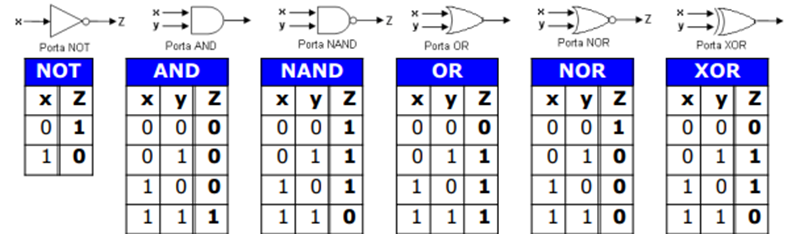
\includegraphics[width=1\linewidth]{Porte Logiche.png}
    \caption{\textbf{Porte Logiche}}
\end{figure}
\newpage
\begin{figure}[h]
    \centering
    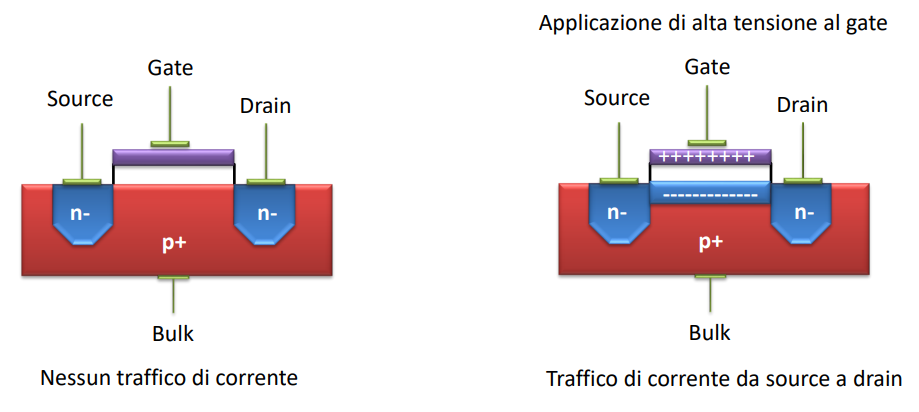
\includegraphics[width=1\linewidth]{NMOS.png}
    \caption{\textbf{nMOS}}
\end{figure}

\begin{figure}[h]
    \centering
    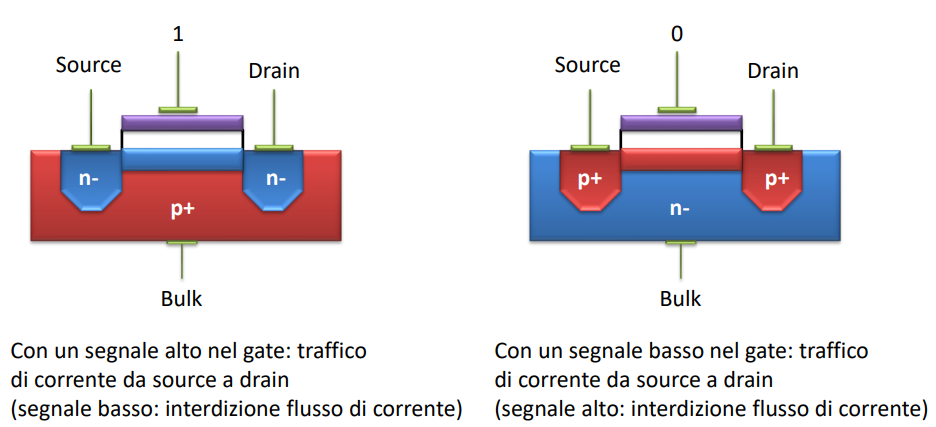
\includegraphics[width=1\linewidth]{cMos.png}
    \caption{\textbf{CMOS: nMOS - pMOS}}
\end{figure}

\newpage
\subsection{Rete Combinatoria}
Una rete è una interconnessione di componenti attivi,le porte, collegati tra loro mediante componenti passivi, le linee. \par\medskip\noindent
Una rete combinatoria è un circuito elettronico in grado di elaborare, in modo automatico, funzioni binarie di una o più variabili binarie.
Formalmente una rete \textbf{combinatoria} è definita come un dispositivo con n linee di ingresso ed m linee di uscite per cui i segnali di uscita dipendono unicamente dai segnali di ingresso.\par\medskip\noindent
\textit{Osservazione}. In una rete combinatoria non sono presenti cicli né cappi Nelle reti combinatorie non può avvenire che gli stessi ingressi forniti in istanti diversi diano luogo ad uscite diverse. \par\medskip\noindent
Uno schema circuitale è un collegamento di porte (rappresentate in maniera grafica) tramite linee. \textbf{Ci sono tre tipi di linee:}
\begin{enumerate}
    \item linee di ingresso, ognuna etichettata con una delle n variabili booleane.
    \item linee di uscita, ognuna etichettata con una delle m variabili di uscita.
    \item linee interne, ciascuna delle quali collega l'uscita di una porta con l'ingresso di un'altra porta.
\end{enumerate}
\textbf{Vincoli:}
\begin{itemize}
    \item Ogni ingresso di ogni porta deve esserecollegato ad una linea di ingresso oppure aduna linea interna.
    \item  L'uscita di ogni porta deve essere collegata aduna linea di uscita oppure ad una lineainterna.
    \item Il collegamento di porte tramite linee nondeve dare luogo a cicli
\end{itemize}
\par\medskip\noindent
Una rete combinatoria può essere vista come un dispositivo in grado di soddisfare una tabella, la tabella della verità, che per ognuna delle 2n combinazioni possibili relative agli n valori di, x2
,.., xn) indica gli m valori di uscita (z1, z2, .., zm).\par\medskip\noindent
\textit{Osservazione}. Ad ogni rete caratterizzata da una tabella con n ingressi ed m uscite corrisponde un gruppo di m espressioni booleane (e viceversa).
\newpage
\subsubsection{Caratteristiche Progettuali}
Tra i parametri principali nel progetto di una rete combinatoria, è opportuno considerare:
\begin{itemize}
    \item \textbf{L’assorbimento di energia} (che stabilisce un limite complessivo al numero di porte utilizzabili).
    \item \textbf{Il ritardo} (che determina la velocità di calcolo). La velocità di calcolo della rete combinatoria. Varia in base alla profondità della rete (di solito si considera un tempo costante perché la rete combinatoria ha una profondità finita).
    \item \textbf{Il costo di realizzazione}. Dipende dal numero di transistor impiegati che cambia a seconda della tecnologia usata, della funzione da soddisfare e il numero di ingressi. Es.: la porta NOT è costituita da 1 transistor, NAND o NOR 2 transistor; AND e OR 3 o 4 transistor; altre porte: \(>\) 4 transistor\par\medskip\noindent
\end{itemize}
\subsubsection{Decoder}
Il decodificatore è una rete combinatoria che trasforma parole associate a codifiche strette in parole associate a codifiche lasche (le linee di uscita sono in numero maggiore rispetto le linee di ingresso).\par\medskip\noindent
Un decodificatore è una rete combinatoria con m linee di ingresso e n=2m linee di uscita. Logicamente il decodificatore riconosce una stringa (es.: una locazione di memoria o unaistruzione).\par\medskip\noindent
Il \textbf{decodificatore} è usato, ad esempio, per identificare una cella di memoria.\par\medskip\noindent

\subsubsection{MUX}
I \textbf{codificatori} sono una famiglia di reti combinatorie che trasformano parole codificate in una codifica lasca in parole d’uscita rappresentate in codifica stretta. \par\medskip\noindent
In generale un codificatore è una rete combinatoria che ha n linee di ingresso e m = \(log2(n) \) linee di uscita, cioè vi è la produzione della codifica binaria dell’indice dell’unica linea di ingresso attiva. \par\medskip\noindent
Logicamente il codificatore è un generatore di codici (es.: dei comandi).

\newpage
\subsection{Circuiti Elementari}
\subsubsection{Addizionatore (Adder)}
L’\textbf{addizionatore} è una rete combinatoria che consente l’operazione di somma tra due
operandi (addendi). \par\medskip\noindent
La rete combinatoria associata ad un addizionatore può essere realizzata mediante una tecnica di decomposizione. Questo perché l’addizione di due numeri binari può essere vista come la somma di due bit alla i-esima posizione (\(xi\) e \( yi\)) ai quali va aggiunto il \textbf{riporto} \((ri)\) per ottenere un \textbf{risultato} \((zi)\) ed un eventuale \textbf{riporto} \((ri+1)\) per le\textbf{ cifre successive}.
\begin{figure}[h]
    \centering
    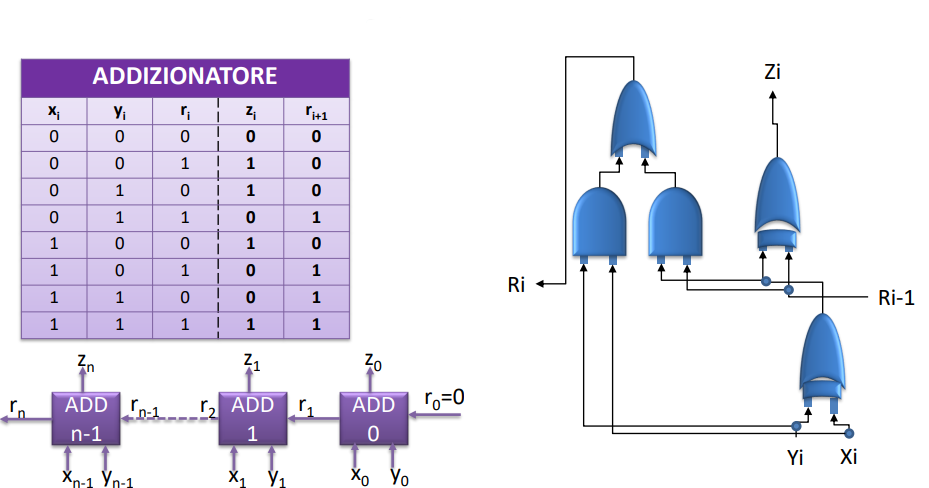
\includegraphics[width=0.75\linewidth]{Addizionatore.png}
    \caption{\textbf{Adder}}
\end{figure}

\subsubsection{Sottrattore}
Il sottrattore è una rete combinatoria che permette la sottrazione tra due operandi (minuendo e sottraendo).\par\medskip\noindent
Anche in questo caso è possibile fare riferimento ad una struttura modulare.
All’i-esimo bit del minuendo (\(xi\)) va sottratto sia il sottraendo (\(yi\)) sia ilbit di prestito (\(pi\)) della posizion eprecedente per poi generare il bit risultante (\(zi\)) ed il bit del prestito (\(pi+1\)) per le cifre successive.\par\medskip\noindent
\textbf{Nel concreto} la realizzazione di un sottrattore può essere effettuato con una circuiteria differente da quella vista. \par\medskip\noindent
L’operazione di sottrazione \(z=m-s\) si riduce alla espressione equivalente \(z=(m+(-s))\)
Si utilizza un complementatore ed un addizionatore che prende in input come addendi il numero complementato ed il valore 1. L’operazione di sottrazione si ottiene aggiungendo il minuendo.


\begin{figure}[h]
    \centering
    \begin{subfigure}[b]{0.40\textwidth}
        \centering
        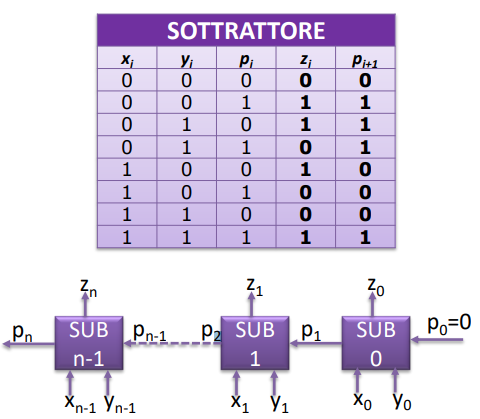
\includegraphics[width=\textwidth]{Sottrattore.png}
        \caption{\textbf{Tabella}}
    \end{subfigure}
    \hfill % separatore orizzontale
    \begin{subfigure}{0.40\textwidth}
        \centering
        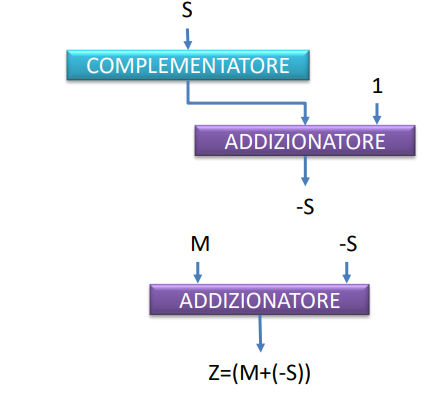
\includegraphics[width=\textwidth]{Schema.png}
        \caption{\textbf{Schema Logico}}
    \end{subfigure}
    \caption{\textbf{Il Sottrattore}}
    \label{fig:main}
\end{figure}

\subsubsection{Comparatore Logico}
Il \textbf{comparatore} è una rete combinatoria che ha una unica linea di uscita che vale 1 se il numero x, di n bit, applicato in ingresso risulta maggiore o uguale (in senso algebrico) al numero y, di n bit, anch’esso preso in ingresso, con cui si effettua il confronto.
Anche per tale componente è possibile fare riferimento ad una struttura modulare. \par\medskip\noindent
Altresì, invece, è possibile realizzare un comparatore logico utilizzando n porte XOR, a cui in ingresso sono associati gli i-esimi bit dei valori da comparare, le cui uscite sono collegate ad una porta OR.\par\medskip\noindent
In questo caso, infatti, è necessario stabilire solamente se le stringhe binarie sono uguali o diverse. Un comparatore logico determina il risultato finale in tempo costante O(1).

\begin{figure}[h]
    \centering
    \begin{subfigure}[b]{0.40\textwidth}
        \centering
        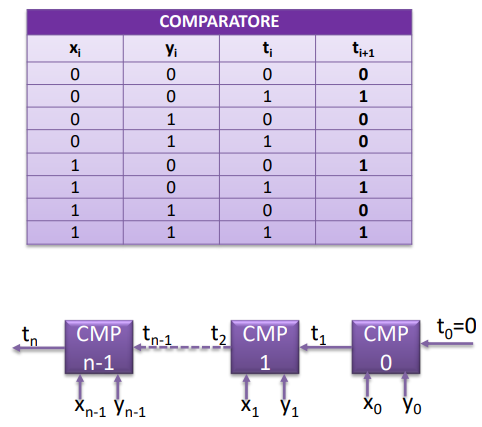
\includegraphics[width=\textwidth]{comparatore.png}
        \caption{\textbf{Tabella}}
    \end{subfigure}
    \hfill % separatore orizzontale
    \begin{subfigure}[b]{0.45\textwidth}
        \centering
        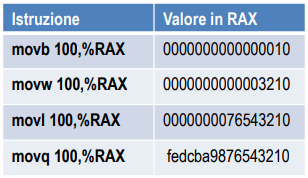
\includegraphics[width=\textwidth]{image.png}
        \caption{\textbf{Schema Logico}}
    \end{subfigure}
    \caption{\textbf{Il comparatore Logico}}
\end{figure}

\newpage
\section{Macchina di Von Neumann}
\subsection{Breve Storia}
Nel 1642 \textbf{Pascaline}. Sistema per il calcolo di addizioni e sottrazioni creato da Pascal
Nel 1672 \textbf{Stepped Reckoner}, ossia la calcolatrice meccanica a quattro operazioni (addizione, sottrazione, prodotto e divisione) inventata da Von Leibniz. Sistema per il conteggio di informazioni con caratteristiche comuni (tabulatore). Usato da Hollerith per il censimento statunitense del 1890. Uso di un ordinatore (sorter) e schede perforate.\par\medskip\noindent
\textbf{ENIAC} (Electronic Numerical lntegrator And Computer). L’elaboratore ENIAC era costituito da
18.000 valvole termoioniche e 1.500 relè, pesava 30 tonnellate e consumava 140KW di energia. Dal punto di vista dell'architettura, la macchina era dotata di 20 registri, ciascuno dei quali in grado di memorizzare un numero decimale a 10 cifre. ENIAC veniva programmato regolando 6000 interruttori multiposizione e connettendo una moltitudine di prese con una vera e propria foresta di cavi.

\subsection{Macchine Programmabili}
Famiglia di calcolatori con architettura che consente l’esecuzione di programmi memorizzati in memoria. \textbf{Un programma }è un insieme di istruzioni elaborate sequenzialmente (a meno di eventuali salti). \par\medskip\noindent
Nel 1945 fu presentato \textbf{un modello di elaboratore generale} grazie a John von Neumann e Hermann Goldstine. \par\medskip\noindent
Il modello di \textbf{“macchina di von Neumann”} (o “macchina di Princeton”) prevedeva che i dati e le istruzioni fossero archiviate nella stessa memoria (architettura adottata dall’elaboratore EDSAC del 1949). Oltre al calcolo matematico, nel programma era possibile effettuare salti in accordo a precise condizioni. Tale modello, per quanto perfezionato nei singoli componenti, è fino oggi il punto di riferimento per la progettazione di un qualsiasi elaboratore elettronico.
\begin{figure}[h]
    \centering
    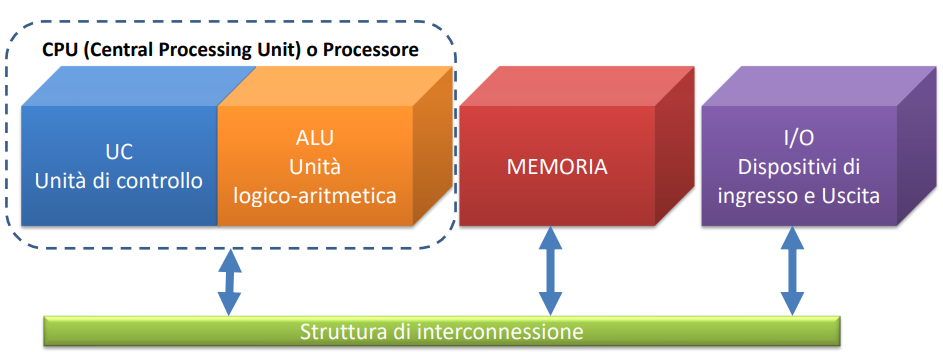
\includegraphics[width=0.75\linewidth]{von neumann.png}
    \caption{\textbf{La CPU}}
\end{figure}
\newpage
\subsection{CPU}
\subsubsection{Unità di Controllo}
\textbf{L’Unità di Controllo} (Control Unit, \textbf{CU}) è predisposta a scandire le sequenze di operazioni elementari necessarie ad eseguire ogni singola istruzione. Le istruzioni devono essere prelevate dalla memoria, e trasferite alla circuiteria interna all’Unità di Controllo.\par\medskip\noindent
La \textbf{circuiteria dell’unità di controllo} deve riconoscere e generare i comandi atti all’esecuzione dell’istruzione (attivazione della struttura di interconnessione, passaggio dei dati e degli indirizzi in memoria, …). 
\begin{figure}[h]
    \centering
    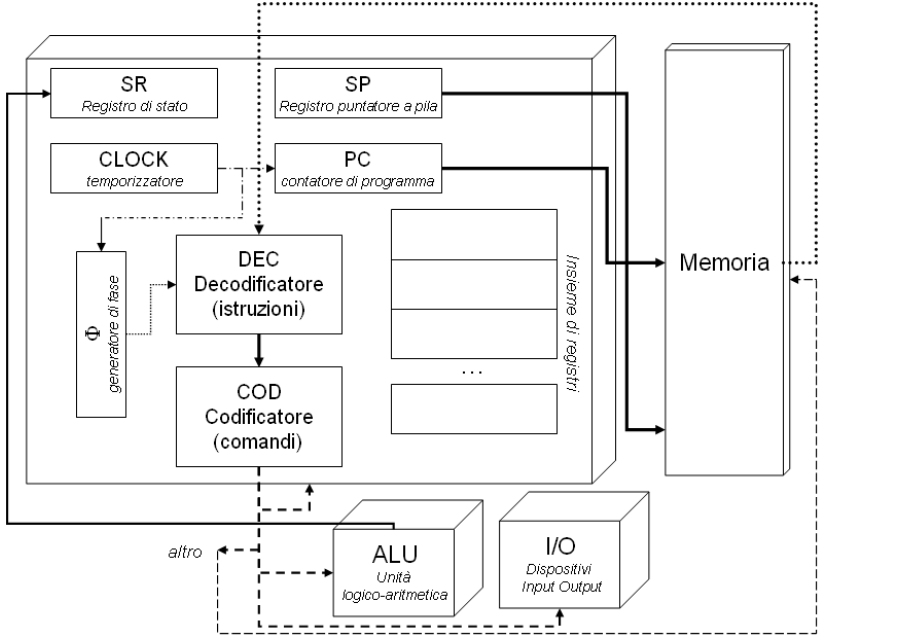
\includegraphics[width=0.75\linewidth]{image1.png}
    \caption{\textbf{Unità di controllo}}
\end{figure}

\noindent Nell’Unità di Controllo sono presenti dei registri e le differenze principali tra i
essi e le celle di memoria è l’esiguo numero dei primi (sono realizzati con componenti costosi e performanti) e la loro presenza all’interno della CU: c’è una vicinanza e uno scambio di informazione diretto e rapido.\par\medskip\noindent
I \textbf{registri possono essere classificati} come registri ad \textbf{uso generale} o ad \textbf{uso speciale}.
\newpage
\noindent I registri ad \textbf{uso speciale} sono :
\begin{enumerate}
    \item Il Contatore di Programma (\textbf{Program Counter}, PC): è un registro contatore preselezionabile incrementato ad ogni periodo di clock, contenente l’indirizzo della cella di memoria dove è memorizzata l’istruzione da eseguire.
    \item Il Registro di Stato (\textbf{Status Registe}r, SR o Processor Status Word, PSW): contiene informazioni che caratterizzano lo stato dell’Unità Centrale, tra cui, ad esempio, quelle relative all’ultima operazione eseguita (i condition codes provenienti dalla ALU).
    \item Il Puntatore alla Pila (\textbf{Stack Pointer}, SP): contiene l’indirizzo della cima della pila (o canasta) cioè la zona di memoria usata per il passaggio di parametri tra funzioni. \par\medskip\noindent 
\end{enumerate}
Il \textbf{Generatore di Fase} (tipicamente realizzato con un registro contatore) scandisce le fasi delle operazioni elementari eseguite dalla CU che possono essere così schematizzate:
\begin{itemize}
    \item  \textbf{Caricamento} (\textit{FETCH}): lettura dalla memoria della parola puntata dal PC. In questa fase la Memoria Centrale ed il codificatore presente nella CU si connettono per consentire il trasferimento dell’istruzione.
    \item  \textbf{Decodifica} (\textit{DECODE}): riconoscimento del tipo di istruzione e del modo di riferimento degli operandi. Non vi è alcuna connessione con componenti esterni perché il decodificatore è interno alla CU.
    \item \textbf{Esecuzione} (\textit{EXECUTE}): esecuzione dei comandi definiti dal codice operativo dell’istruzione. Vi è connessione con tutte le unità richieste. Mentre le prime due fasi sono uguali per ogni istruzione, la fase di esecuzione varia in relazione dell’operazione coinvolta (es.: una moltiplicazione impiega più tempo di una addizione; più un modo di indirizzamento è complesso più si impiega tempo a reperire gli operandi).
    \item \textbf{Spostamento} (\textit{MOVE}): esegue una movimentazione di dati (es.: si rimette in memoria il risultato di una istruzione aritmetica).\par\medskip\noindent 
\end{itemize}
L’\textbf{elaborazione} di una istruzione consta nella successione di fasi che si ripete continuamente all’atto dell’accensione della macchina.\par\medskip\noindent
Una istruzione è sempre eseguita in queste fasi ma comprende un numero di cicli macchina variabile dipendenti, ad esempio, dal tipo di operazione, dal numero di accessi in memoria o alle unità di I/O. Ogni ciclo macchina, infatti, è implementato mediante una successione di un piccolo numero di operazione elementari eseguite in circuiti diversi sotto il controllo del transcodificatore. Ogni \textbf{operazione elementare} occupa un periodo di clock e pertanto la durata di una istruzione dipende dal numero di accessi alla memoria, all’esterno della CPU e dal numero di operazioni elementari richieste. \par\medskip\noindent
Una volta che l’istruzione è stata caricata viene passata al \textbf{transcodificatore} (cioè il decodificatore delle istruzioni connesso col codificatore dei comandi) che riconosce l’istruzione e genera opportuni comandi per eseguire l’istruzione stessa.\par\medskip\noindent
\textit{Un esempio Pratico: }\textbf{ADD 0x300,0x100,0x200}
\begin{itemize}
    \item In fase di \textbf{fetch} si preleva l’istruzione dalla Memoria Centrale e si incrementa il PC.
    \item In fase di \textbf{decode}, il decodificatore riconosce l’addizione. Il codificatore, a sua volta, invia dei comandi (dei segnali elettrici) lungo le linee di ingresso della ALU che specificano il tipo di operazione che questa deve offrire.
    \item In fase di \textbf{load}, contestualmente il codificatore lancia dei segnali per prendere gli operandi in memoria alla locazione 0x100 e poi 0x200.
    \item In fase di execute, una volta reperiti gli operandi si deve generare la connessione con la ALU disconnettendo la memoria.
    \item La \textbf{ALU esegue l’operazione}.
    \item  In fase di \textbf{movement}, si riattiva la linea con la Memoria Centrale per trasferire il risultato nella locazione 0x300.\par\medskip\noindent
\end{itemize}
L’insieme dei \textbf{registri ad uso generale} è anche denominato FR (\textbf{File Register}, archivio di registri); tali registri sono utilizzati per memorizzare, all’interno dell’Unità Centrale, i risultati temporane provenienti dall’ALU e le informazioni di controllo, allo scopo di diminuire il numero di accessi alla Memoria Centrale e di velocizzare il processo di elaborazione.\par\medskip\noindent 
\subsubsection{ALU}
L’\textbf{Unità Logico-Aritmetica} è il componente che si occupa di effettuare operazioni logiche ed aritmetiche. Per il funzionamento di questa unità di solito sono impiegati un insieme di registri ad uso speciale che servono a contenere gli operandi e il risultato delle operazioni. \par\medskip\noindent
I \textbf{registri speciali} contenuti nella ALU, denominati \textbf{accumulatori}, sono trasparenti al programmatore (cioè il contenuto non può essere modificato dal programmatore mediante istruzioni) e svolgono la funzione di ospitare gli operandi prima e durante l’esecuzione o i risultati dopo l’esecuzione.\par\medskip\noindent
Gli \textbf{accumulatori} hanno un ruolo fondamentale per l’indirizzamento implicito: sono i registri in cui implicitamente vengono mandati gli operandi nel momento in cui si ricorre ad una istruzione logico-aritmetica.\par\medskip\noindent
Oltre agli accumulatori sono presenti delle \textbf{linee di ingresso} che individuano la funzione/operazione che deve essere attivata (le operazioni principali sono: ADD, NEG,
AND, OR, COMP, TESTB, SHIFT) e delle linee di uscite su cui è ricondotto il risultato. Inoltre ci sono delle linee di uscita denominate condition code o flags che riportano informazioni relative all’ultima operazione eseguita. \par\medskip\noindent
Oltre agli accumulatori la ALU ha anche un registro speciale detto registro degli errori nel quale sono riportate situazioni non risolvibili (es.: divisione per zero, radice quadrata di un numero negativo) e che grazie al quale è possibile attivare un’interruzione interna.
\textbf{La CU e la ALU identificano la CPU dell’elaboratore elettronico (il ‘cuore’ della macchina).} Col tempo si è provveduto a realizzare ALU specifiche, denominate coprocessori matematici (o ALU Attaccata), che eseguono funzioni complesse come i calcoli in virgola mobile (MULF, DIVF,COMPF,…) con un set di istruzioni dedicato non presente nel set di istruzioni della macchina. \par\medskip\noindent
Sebbene questa strategia ormai è stata abbandonata, includendo le funzionalità complesse direttamente nella \textbf{ALU-Nativa}, è tuttavia una pratica utilizzata nel caso in cui si voglia aggiungere nuove ALU che fanno operazioni che l’ALU-Nativa non svolge. In questo caso l’\textbf{ALU attaccata} è vista come un dispositivo I/O.\par\medskip\noindent
\subsection{Memoria Centrale}
\subsubsection{RAM}
\textbf{RAM (Random Access Memory)}: Memorie volatili, cioè che perdono le informazioni in mancanza della tensione di alimentazione, il cui accesso a ciascuna locazione avviene in tempo costante.
\begin{itemize}
    \item \textbf{SRAM} (Static RAM): Memorie statiche nelle quali l’informazione è memorizzata nell’equivalente di un latch D.
    \item  \textbf{DRAM} (Dynamic RAM) Memorie dinamiche nelle quali l’informazione è memorizzata in un condensatore. Anche in presenza della tensione di alimentazione l’informazione contenuta in ogni cella è conservata per un breve periodo di tempo (dell’ordine di grandezza di 2 ms), passato il quale il contenuto deve essere ripristinato: questo avviene ciclicamente tramite un’operazione di “rinfresco” (refresh) che viene effettuata dal sistema.
    \item \textbf{SDRAM} (Synchronous DRAM) consente una maggiore flessibilità di impiego permettendo, grazie ad un apposito registro in uscita, di modificare il dato contenuto in una cella mentre si sta utilizzando il vecchio dato. Una ulteriore evoluzione della SDRAM è la \textbf{DDR} (Double Data Rate) che, come indica il nome, consente di operare a frequenza doppia potendo essere pilotata sia sul fronte di salita che sul fronte di discesa del clock.
\end{itemize}

\subsubsection{ROM}
\textbf{ROM (Read Only Memory)}: Memorie di tipo non volatile che hanno la capacità di conservare l’informazione indipendentemente dalla presenza o meno della tensione di alimentazione. Sono memorie programmate dal costruttore e non sono modificabili dall’utilizzatore: è possibile solo la lettura dei dati contenuti. Anche in questo caso l’accesso ad ogni locazione avviene in tempo costante.
\begin{itemize}
    \item  \textbf{PROM} (Programmable ROM). Si tratta di memorie sulle quali l’utilizzatore può scrivere i dati una sola volta, utilizzando un apposito dispositivo di registrazione che brucia dei fusibili.
    \item \textbf{EPROM} (Erasable Programmable ROM). Sono memorie nelle quali l’utilizzatore può memorizzare i dati anche più volte, utilizzando appositi dispositivi di cancellazione (a raggi ultravioletti).
    \item \textbf{EEPROM} (Electrically Erasable PROM) o \textbf{EAROM} (Electrically Alterable ROM). Sono memorie EPROM nelle quali la cancellazione si può fare per via elettrica ma di solito è globale (coinvolge cioè tutti i dati registrati).\par\medskip\noindent
\end{itemize}
\subsubsection{Memoria Centrale}
La Memoria Centrale è una memoria volatile di tipo RAM (di tipologia DDR) costituita da tante locazioni (o celle) ciascuna delle quali può immagazzinare una stringa binaria di lunghezza finita \textit{n}\par\medskip\noindent
Le stringhe presenti in Memoria Centrale possono essere: \textbf{istruzioni}, \textbf{operandi} o \textbf{indirizzi}. \par\medskip\noindent
Le locazioni della Memoria Centrale sono numerate in sequenza da 0 a \(2m-1\) (con m dimensione massima della memoria) e tale numero prende il nome di indirizzo della cella.\par\medskip\noindent 
\par\medskip\noindent L’\textbf{indirizzo} specifica univocamente una locazione. Si accede a qualsiasi locazione con lo stesso tempo (il tempo di accesso ai dati non varia in relazione alla posizione).\par\medskip\noindent
La Memoria Centrale presenta delle aree riservate, in cui risiedono delle informazioni basilari utili al funzionamento della macchina (kernel del Sistema Operativo), ed altre in cui, per comodità sono riservate per operazioni particolari (\textbf{stack}, zona per trasferimento I/O,…).\par\medskip\noindent
La \textbf{Memoria Centrale}, per motivi progettuali ha \textbf{locazione di memoria di lunghezza 8bit}. In ogni caso nel momento in cui si stabilisce la lunghezza della parola si realizza una rete combinatoria che permette il prelievo di tante locazioni contigue quante necessarie per raggiungere la lunghezza della parola.\par\medskip\noindent
Ad esempio se il processore ha una parla di 32bit la circuiteria durante la fase di fetch preleverà (per default) 4 celle contigue in un solo istante.\par\medskip\noindent
La produzione di parole di 8bit non è solo legato a motivi progettuali ma consente anche il prelievo di dati di tipo \textit{byte} (8bit), \textit{halfword} (16bit), \textit{word} (32bit) nella macchina a 32bit (8,32,64 in quelle a 64bit); lunghezze intermedie avvengono manipolando i dati prelevati aventi maggiore lunghezza (mascheramento).\par\medskip\noindent
I dati in memoria possono avere \textbf{due tipi di ordinamento }(endian): la numerazione comincia a partire dall’estremo più “grande” (cioè dal byte più significativo) è chiamato \textbf{big endian} usato nei protocolli internet. In contrapposizione c’è il sistema \textbf{little endian}, usato ad esempio in Intel, Digital, Motorola, IBM, SUN (big endian), MIS può essere impostato in entrambe le organizzazioni.\par\medskip\noindent
Per poter interagire con la Memoria Centrale è necessario che ci siano:
\begin{itemize}
    \item \textbf{linee di ingresso} che specificano un indirizzo (in alcuni testi si fa riferimento al registro MAR, memory address register).
    \item \textbf{linee di uscita} per poter inviare o trasferire il dato (in alcuni testi si fa riferimento al registro MDR, memory data register).
    \item \textbf{un segnale di controllo} (generato dalla CU) per la lettura o la scrittura del dato.\par\medskip\noindent
\end{itemize}
È prevista, pertanto, una architettura costituita da un \textbf{decodificatore} che riceve in ingresso 
l’indirizzo della locazione di memoria alla quale si vuole accedere ed una linea che abilita questa a porre il suo contenuto in uscita dalla memoria o trascrivere in essa il dato da memorizzare.\par\medskip\noindent
Una organizzazione di questo tipo è impraticabile nel caso in cui la memoria abbia una grande dimensione. Con indirizzi, di lunghezza m, è possibile indirizzare 2m celle di memoria. Nel caso il valore di m sia grande (superi il valore 10) una architettura gestita da un singolo decoder è da escludere.\par\medskip\noindent
Per questo si ricorre ad una suddivisione logica della Memoria Centrale (multidimensione). \textbf{La Memoria Centrale} è suddivisa logicamente in banchi (bank, o piastre) e blocchi (block). L’\textbf{indirizzo} è suddiviso in campi ognuno con un significato associato ai banchi, blocchi e locazioni presenti e per ogni campo è presente un proprio decodificatore.\par\medskip\noindent
\textit{Ad Esempio:} nel caso di due banchi con quattro blocchi avremo una suddivisione in
tre campi: il \textbf{primo campo} di un bit indicante il banco; \textbf{il secondo} di due bit il blocco; il terzo dei rimanenti bit la posizione in cui risiede la locazione.
\newpage
\begin{figure}[t]
    \centering
    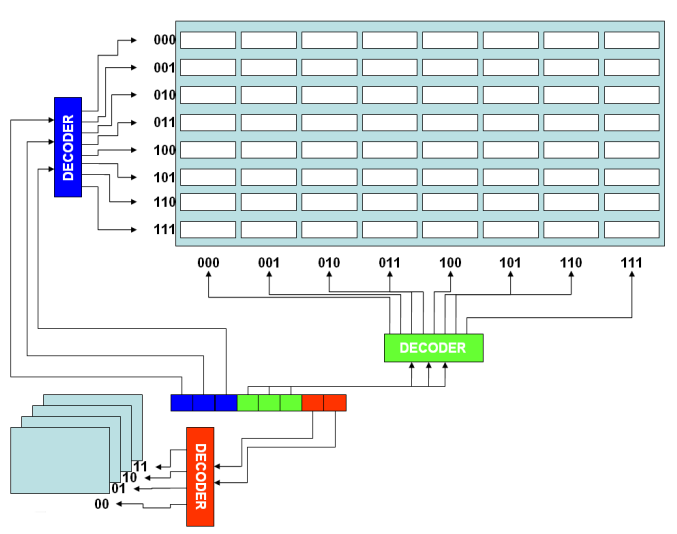
\includegraphics[width=0.75\linewidth]{Memoria Centrale .png}
    \caption{Suddivisione logica della memoria centrale}
\end{figure}
\begin{figure}[h]
    \centering
    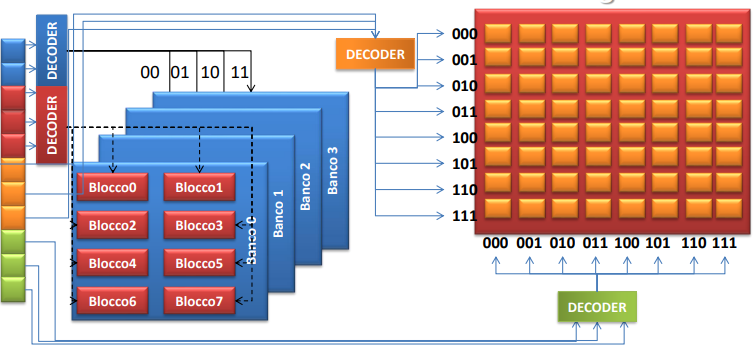
\includegraphics[width=0.75\linewidth]{Memoria Centrale.png}
    \caption{Memoria Centrale} 
\end{figure}
\newpage
\subsection{Dispositivi di Input ed Output}
I \textbf{dispositivi di input/output} (dispositivi di I/O o periferiche) consentono di collegare l’elaboratore, ed in particolare la Memoria Centrale con il mondo esterno (persone o altri dispositivi). Esistono numerosi tipi di dispositivi di I/O con caratteristiche molto varie che comportano problemi relativi alla conversione tra rappresentazione interna ed esterna dell’informazione.\par\medskip\noindent
Le \textbf{velocità di trasferimento} sono inferiori a quelle possibili all’interno delle altre componenti (CPU, Memoria Centrale) a causa della natura tecnologica di fabbricazione (componenti meccanici,…) e quindi l’uso delle periferiche comporta problemi di sincronizzazione e di adattamento della velocità.\par\medskip\noindent
Quando c’è un trasferimento dati è opportuno che il dispositivo coinvolto e il processore operino in modo coordinato mediante un insieme di regole: \textbf{il protocollo}.\par\medskip\noindent
Il protocollo consente l’interazione tra dispositivo (identificato da un indirizzo) e la Memoria Centrale sotto il controllo del Processore. Il \textbf{dispositivo} deve essere in grado di operare qualora il processore ne richieda l’intervento. Il \textbf{processore} deve eseguire le operazioni che consentono il trasferimento solo quando il dispositivo è pronto.\par\medskip\noindent
Nel\textbf{ protocollo di input} una periferica vuole inviare dati all’elaboratore. I dati devono essere stipati in Memoria Centrale.
Il protocollo prevede:
\begin{itemize}
    \item  L’individuazione del dispositivo di input che vuole inviare i dati
    \item  La ricerca di un’area libera in cui stipare i dati
    \item  Il prelievo del dato 
\end{itemize}
\textit{Ad esempio} = si richiede l’immissione di un valore da tastiera:
\begin{enumerate}
    \item Si individua nella tastiera il dispositivo che vuole inviare i dati.
    \item Si trova un’area libera della Memoria Centrale per stipare l’informazione.
    \item Avviene il prelievo del dato immesso da tastiera residente in una memoria interna al dispositivo per essere spostato in Memoria Centrale.
\end{enumerate}
\newpage \noindent Nel \textbf{protocollo di output} una periferica ospita i dati prodotti dall’elaboratore eli rielabora in relazione alla propria funzione (stampante, memoria di massa, controreazione nei joystick).
Il protocollo prevede:
\begin{itemize}
    \item L’individuazione del dispositivo che deve ricevere i dati
    \item Dei controlli sul dispositivo.
    \item L’invio dei dati\par\medskip\noindent
\end{itemize}
\textit{Ad esempio} = si richiede il salvataggio di un'immagine su un disco magnetico:
\begin{enumerate}
    \item Si individua il disco magnetico
    \item Si trova un’area libera per stipare l’informazione e si svolgono controlli (ad esempio si controlla il nome del file per evitare che ci siano duplicati).
    \item Avviene il trasferimento dei dati dalla Memoria Centrale al disco magnetico
\end{enumerate}
Per interagire con il processore ogni dispositivo deve essere interconnesso ad un \textbf{modulo di I/O} (o interfaccia I/O o controller), cioè una rete sequenziale che colloquia con il processore inviando e ricevendo (tramite un bus di I/O) i segnali che, secondo il protocollo, controllano le operazioni di trasferimento.\par\medskip\noindent
Il protocollo di I/O pertanto è caratteristico dell’elaboratore, in quanto determinato dal modo di operare del processore, cioè dall’insieme di istruzioni di cui il processore può disporre per i trasferimenti. Questo vuol dire che i diversi dispositivi esterni collegati allo stesso elaboratore devono rispettare tutti lo stesso protocollo di I/O, indipendentemente dalla natura delle informazioni trasferite a dalla struttura fisica del dispositivo. Solamente in seguito il dispositivo da il giusto significato al codice ricevuto. \par\medskip\noindent
\textbf{Schema di un dispositivo di input}. Si evidenzia la sotto-rete (controller) che non
dipende dal dispositivo e che è interessata nel colloquio con il processore. (Il controller è la parte più significativa dell’interfaccia di I/O).
\begin{figure}[h]
    \centering
    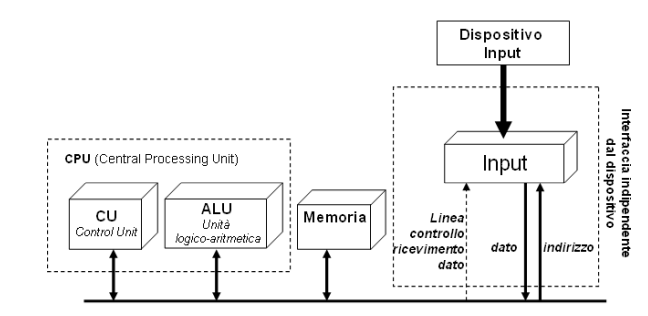
\includegraphics[width=0.50\linewidth]{input.png}
    \caption{Controller}
\end{figure}
\begin{figure}[t]
    \centering
    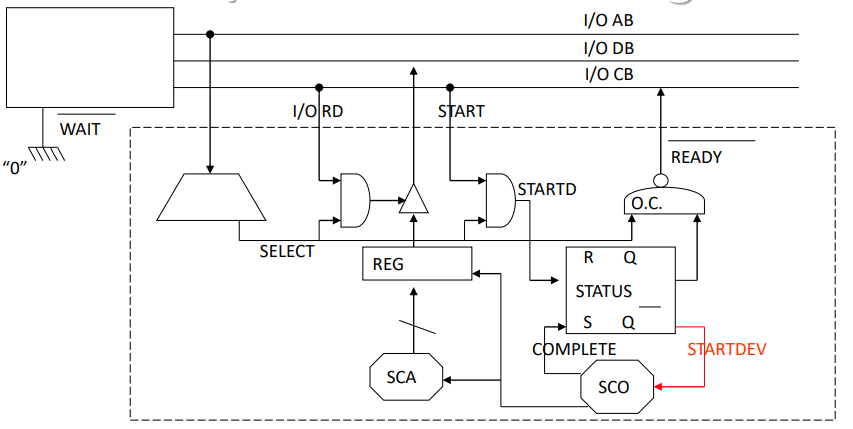
\includegraphics[width=1\linewidth]{controller.png}
    \caption{Controller Nel Dettaglio}
\end{figure}
\newpage
\textbf{Protocollo INPUT}
\begin{enumerate}
    \item  Il processore invia sull’I/O Address bus l’indirizzo del dispositivo e ne esamina lo stato tramite la linea di controllo READY.
    \item Se il dispositivo non è pronto il processore deve attendere e tornare al punto 1 (in alternativa procede elaborando un’altra istruzione e poi ripete il punto 1); se è pronto va la punto 3
    \item Il processore avverte il dispositivo che può prendere un dato (seleziona il dispositivo tramite le linee indirizzi e invia il segnale START). START resetta il flip-flop STATUS e in tale stato rimane per tutta la durata delle operazioni di produzione del dato da parte del dispositivo
    \item Quando il dato è stato prodotto ed è disponibile in REG, il dispositivo genera il segnale COMPLETE, settando STATUS (READY=0).
    \item Nel frattempo il processore, in attesa del dato, esamina il flip flof STATUS campionando il segnale READY
    \item Se READY= 1 il processore deve attendere e tornare al punto 5.
    \par\medskip\noindent Se READY= 0 il processore invia il segnale di controllo IO/RD per trasferire il dato presente in REG all’interno della locazione di memoria libera (cioè deputata ad ospitare il valore).
\end{enumerate}
\newpage
\textbf{Protocollo OUTPUT}
\begin{enumerate}
    \item Il processore invia sull’I/O Address bus l’indirizzo del dispositivo e ne esamina lo stato tramite la linea di controllo READY.
    \item Se il dispositivo non è pronto il processore deve attendere e tornare al punto 1 o svolgere un’altra istruzione. Se è pronto va al passo 3
    \item Se READY=0 il processore trasferisce il contenuto di una locazione di memoria nel registro di interfaccia del dispositivo (mediante il segnale di controllo I/O WR)
    \item Il processore avverte il dispositivo che gli ha trasferito un dato inviando il segnale START. START resetta il flip-flop STATUS e in tale stato rimane per tutta la durata delle operazioni di consumo del dato da parte del dispositivo. Quando il dato è stato letto da REG, il dispositivo genera il segnale COMPLETE, settando STATUS (READY=0).
    \item Nel frattempo il processore, in attesa, esamina lo stato di STATUS campionando il segnale READY.
    \item  Se READY= 1 il processore deve attendere e tornare al punto 5.\par\medskip\noindent
    Se READY= 0 il processore può eseguire un’altra istruzione.\par\medskip\noindent
\end{enumerate}
Per \textbf{indirizzare le unità di I/O} e consentire l’accesso al dato da trasferire o recuperare, il processore ricorre ad una delle due seguenti tecniche :
\begin{itemize}
    \item Riservare all’I/O uno spazio di indirizzamento indipendente: si utilizzano specifiche istruzioni nelle quali si fornisce anche l’indirizzo identificativo del dispositivo da utilizzare nell’operazione (\textbf{I/O -CANONICO}).
    \item Riservare una porzione dello spazio di indirizzamento in Memoria Centrale ai dispositivi di I/O, in modo che ogni volta che il processore utilizza un indirizzo di questa porzione (con una tipica istruzione di trasferimento dati cioè senza ricorrere a specifiche istruzioni) in realtà fa riferimento ad un dispositivo di I/O (\textbf{I/O PROGRAMMATO})
\end{itemize}
\newpage
\subsection{Interconnessione tra moduli}
Le informazioni elaborate da un calcolatore elettronico prendono in considerazione delle stringhe binarie che hanno il significato di operando, indirizzo o istruzione.\par\medskip\noindent
Una stringa binaria, o parola (word), è una sequenza di bit di dimensione prefissata che deve essere considerata come unità indivisibile ed è stabilita a priori dal progettista dell’elaboratore. \par\medskip\noindent
Le singole cifre costituenti una parola sono memorizzate in latch e l’insieme risultante è un componente denominato registro (a volte i termini parola e registro si considerano equivalenti).\par\medskip\noindent
Il modo più semplice per realizzare un registro è quello di utilizzare n celle di memoria ed almeno due linee: una (write, W) per selezionare simultaneamente le n celle che compongono la parola e consentire la loro sovrascrittura con nuovi valori; mentre l’altra è di azzeramento (clear, C) del registro, cioè impostando, o ‘pulendo’, il contenuto di ogni latch con il valore 0. \par\medskip\noindent
Il transito di informazione è consentito dai sistemi di interconnessione, cioè delle reti che sono in
grado di trasferire, o meglio duplicare, l’informazione contenuta nei registri.
L’\textbf{interconnessione} punto a punto effettua il trasferimento della parola contenuta in un registro sorgente, Rs, a un registro destinazione, Rd. \par\medskip\noindent
Tutti gli n latch di Rs (linee di uscita) sono legati agli n latch (linee di entrata) di Rd ovviamente predisponendo una linea (transfer o write) di controllo che indica, con il comando 1, il trasferimento di informazione (la sovrascrittura) e con 0 la conservazione del valore corrente nel registro destinazione. \par\medskip\noindent
Il \textbf{multiplexer} è la rete d’interconnessione che consente il trasferimento tra \(m\) registri sorgenti e un registro destinazione prefissato.
\begin{figure}[h]
    \centering
    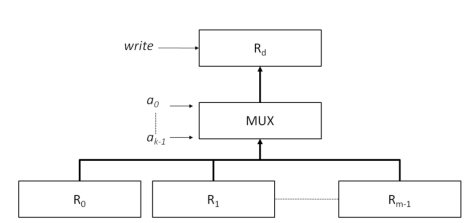
\includegraphics[width=0.50\linewidth]{mux.png}
    \caption{MUX}
\end{figure}
\newpage 
\noindent Il \textbf{demultiplexer} è la rete di interconnessione fatta per favorire il trasferimento tra un registro sorgente e uno degli m registri destinatari.
\begin{figure}[h]
    \centering
    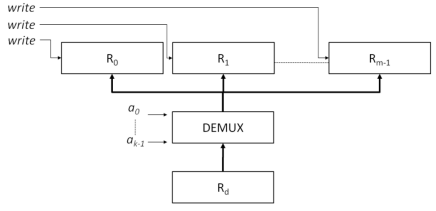
\includegraphics[width=0.5\linewidth]{demux.png}
    \caption{DEMUX}
\end{figure}
\par\medskip\noindent
Le \textbf{reti mesh} sono reti in grado di interconnettere tra loro m registri, o più in generale m componenti.
\begin{figure}[h]
    \centering
    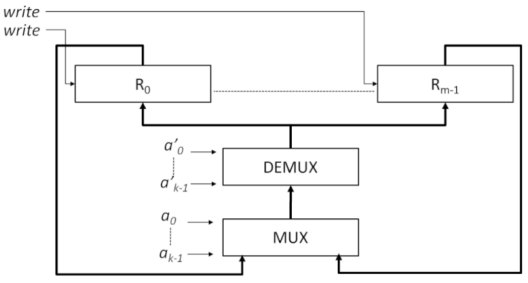
\includegraphics[width=0.5\linewidth]{mesh.png}
    \caption{Mesh}

\end{figure}
\par\medskip\noindent
Il \textbf{bus} è un fascio di k (di solito è uguale o maggiore alla dimensione del
registro) linee. Per il trasferimento è sufficiente attivare la linea di ingresso di selezione (s)
del registro sorgente e quella del registro destinazione.\par\medskip\noindent 
\begin{figure}[h]
    \centering
    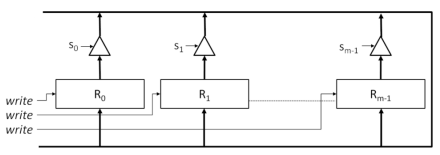
\includegraphics[width=0.5\linewidth]{bus.png}
    \caption{Enter Caption}
\end{figure}
\newpage 
\noindent Il bus sfrutta un buffer tristate, un dispositivo usato per permettere a più porte
logiche di pilotare la stessa uscita, generalmente un bus. Se la linea S ha carica positiva
si consente il passaggio dei dati, da IN a OUT, altrimenti si inibisce il trasferimento.\par\medskip\noindent
\subsubsection{Interconnessione bus}
I primi elaboratori avevano un unico bus chiamato anche bus di sistema. Esso era composto dai 50 ai 100 fili paralleli di rame che si inserivano nella scheda madre e i cui connettori erano distanziati a intervalli regolari per permettere l’inserimento di memorie e schede
di I/O. Attualmente si usano più bus (multi bus): uno specifico tra la CPU e la Memoria Centrale e (almeno) un altro bus per le periferiche.\par\medskip\noindent 
\subsubsection{Interconnessione bus Master/Slave}
Alcune periferiche che si collegano al bus sono attive (\textbf{master}) e possono iniziare un trasferimento dati, mentre altre sono passive (\textbf{slave}) e restano in attesa di una richiesta. \par\medskip\noindent
Quando il processore ordina al controllore di un disco di leggere o di scrivere un blocco, svolge il ruolo di master, e il controllore del disco quello di slave. Successivamente però il controllore
del disco fa da master nel momento in cui ordina alla Memoria Centrale di accettare le parole che sta leggendo dal disco. La Memoria Centrale non può mai svolgere la funzione di master.\par\medskip\noindent
\subsubsection{Interconnessione bus multipli e bus multiplexato}
Il bus consente il transito di operandi, dati e controlli. Il numero di linee che costituisce il bus influenza la progettazione della macchina (costi, organizzazione topologica,…). \par\medskip\noindent
Per aggirare il problema di bus mulitipli si può usare un bus multiplexato. In questa architettura invece di tenere separate le linee d’indirizzo e quelle dei dati, si utilizza un certo numero di linee per entrambi: all’inizio di un’operazione sul bus le linee sono utilizzate per gli indirizzi, mentre in seguito vengono impiegate per i dati.\par\medskip\noindent
ES.: nel caso di una scrittura in memoria le linee d’indirizzo devono essere impostate ai valori corretti e propagate fino alla memoria prima di spedire i dati sul bus.

\subsubsection{Interconnessione bus: arbitraggio centralizzato}
Nel caso di un solo bus e di due o più dispositivi che richiedono contemporaneamente l'uso del bus si ricorre ad un arbitraggio del bus. L'arbitraggio può essere centralizzato o decentralizzato.\par\medskip\noindent
Arbitraggio centralizzato: un arbitro del bus (contenuto nella CPU o esterno ad esso) determina chi è il prossimo dispositivo.\par\medskip\noindent
L'arbitratore del bus, nel caso più semplice sfrutta la tecnica daisy chaining: ha un’unica linea di richiesta (non sa quanti e quali dispositivi hanno richiesto il bus, ma solo che c'è o non c'è almeno una richiesta )\par\medskip\noindent
L'arbitratore abilita l'uso della linea. Il dispositivo di I/O più vicino verifica se ha richiesto l'uso del bus: se si, si impossessa del bus e non consente di trasmettere oltre il segnale di concessione. Se invece non ha fatto richiesta, propaga la concessione sulla linea in direzione del
prossimo dispositivo\par\medskip\noindent
Per evitare che la scelta ricada sempre sulla distanza e non sul tipo di dispositivo si possono usare delle linee di priorità\par\medskip\noindent
Nei sistemi in cui la memoria è collegata al bus principale, la CPU deve competere con tutti i dispositivi di I/O praticamente a ogni ciclo. Di solito la CPU ha la priorità più bassa rispetto gli I/O. I dispositivi di I/O sono obbligati ad acquisire il bus molto velocemente, pena la perdita dei dati in arrivo. I dischi che ruotano ad alte velocità, per esempio, non possono aspettare\par\medskip\noindent
\subsubsection{Interconnessione bus: arbitraggio decentralizzato}
Nell'arbitraggio decentralizzato del bus si usano più linee di richiesta, ciascuna con la
propria priorità. Quando un dispositivo vuole utilizzare il bus invia un segnale lungo la linea di richiesta.\par\medskip\noindent
Tutti i dispositivi monitorano tutte le linee di richiesta in modo che alla fine di ciascun ciclo di analisi del bus ognuno di loro può sapere se era il richiedente con priorità più elevata e se quindi ha diritto a utilizzare il bus durante il ciclo successivo. \par\medskip\noindent
Rispetto al metodo centralizzato questo schema di arbitraggio richiede un maggior numero di linee di bus, ma evita il potenziale costo dell’arbitratore. Un altro limite è che il numero di dispositivi non può superare il numero delle linee di richiesta.
\newpage
\subsection{Macchina Harvard}
La prima data ufficiale in cui si realizzò un modello di elaboratore elettronico fu il 1944 con la “\textbf{macchina di Harvard}”, dal nome del college in cui si trovava il gruppo di lavoro che l’aveva ideata (fu adottata dall’elaboratore MARK). \par\medskip\noindent
La macchina di Harvard era costituita da una Unità di Calcolo, una Unità di Controllo, una Memoria delle Istruzioni, una Memoria Dati ed un modulo per i Dispositivi di input ed output, opportunamente collegati per consentire un flusso di comandi e di controlli che ne permettevano il funzionamento e colloquio reciproco e lo svolgimento di una istruzione ad un colpo di clock.\par\medskip\noindent
La “macchina di Harvard” fu migliorata nel 1982 con un set appropriato, multibus e una serie di registri ad uso generale che consentivano di eseguire ciascuna istruzione di lunghezza fissa a 32bit in un solo colpo di clock.\par\medskip\noindent
Il progetto iniziò nel 1981 per opera di John L. Hennessy dell’Università di Stanford.\par\medskip\noindent
Realizzazione di una architettura di tipo RISC (poche istruzioni e pochi modi di indirizzamento) e in grado di realizzare la tecnica della canalizzazione (pipeline).\par\medskip\noindent
Suddivisione della Memoria Centrale in due parti fisiche (Memoria Istruzioni e Memoria Dati) per garantire l'esecuzione di una istruzione in un solo ciclo di clock.\par\medskip\noindent 
\begin{figure}[h]
    \centering
    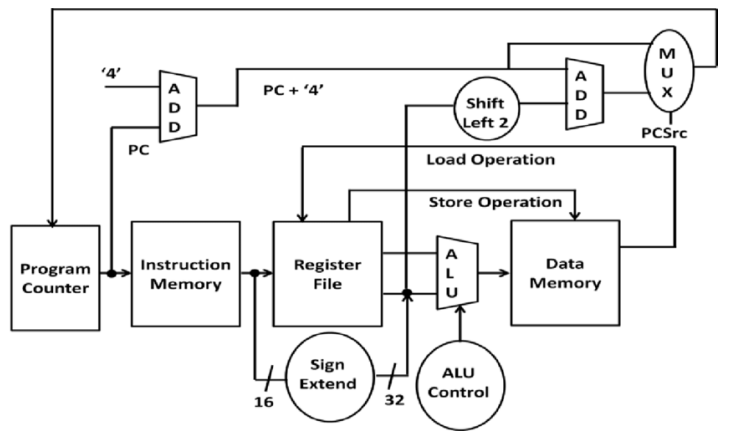
\includegraphics[width=0.75\linewidth]{harvard.png}
    \caption{Enter Caption}
\end{figure}


\newpage
\section{Dal codice sorgente al codice esguibile}
L’esecuzione di un programma è il punto di arrivo di una sequenza di azioni che nella maggior parte dei casi iniziano con la scrittura di un programma in un linguaggio simbolico di alto livello.\par\medskip\noindent
Le azioni principali che compongono tale sequenza nel caso si parta da un linguaggio ad alto livello sono quelle che vedono in gioco il \textbf{compilatore}, l’\textbf{assemblatore} e il \textbf{collegatore}\par\medskip\noindent 
Alcuni calcolatori raggruppano queste azioni per ridurre il tempo di traduzione, ma concettualmente tutti i programmi compilati passano sempre attraverso le fasi mostrate.\par\medskip\noindent
\subsection{Assemblatore}
L’assemblatore converte un programma assembly in un file oggetto, che è una combinazione di istruzioni in linguaggio macchina, di dati e di informazioni necessarie a collocare le istruzioni in memoria nella posizione opportuna. \par\medskip\noindent
Un programma assembly è tradotto in una sequenza di istruzioni (opcode, indirizzi, costanti, ecc.) attraverso il processo di assemblaggio (assembler) costituito da due passi logici successivi ed in parte indipendenti :
\begin{enumerate}
    \item  il programma assembly è letto sequenzialmente, si identificano le istruzioni e i loro operandi, si calcola la lunghezza e si assegna un indirizzo (relativo) a ciascuna istruzione; inoltre, quando è letto un simbolo (un indirizzo simbolico, cioè una etichetta), nome e indirizzo sono inseriti in una tabella dei simboli (symbol table): nome e indirizzo di un simbolo possono essere inseriti nella symbol table in momenti diversi se un simbolo è usato prima di essere definito.
    \item il programma assembly è letto sequenzialmente, a tutti i simboli è sostituito il valore numerico corrispondente presente nella symbol table, a tutte le istruzioni e ai relativi operandi ancora in forma simbolica è sostituito il valore numerico corrispondente (opcode, ecc...).
\end{enumerate}
\textbf{Il processo di assemblaggio prende il nome di assegnazione interna delle locazioni (internal relocate symbol o internal reference)}.
\newpage
\subsection{Compilatore}
Il \textbf{compilatore} trasforma, dopo un controllo sintattico, il programma scritto in un linguaggio ad alto livello in uno in linguaggio assembly, cioè in una forma simbolica che il calcolatore è in grado di capire ma, ancora, non eseguire.\par\medskip\noindent 
Durante la generazione del codice, il compilatore effettua il riordino delle istruzioni cioè quali istruzioni sono trasmesse al processore e in quale ordine (utile nella canalizzazione o per il calcolo parallelo). Infine il compilatore ottimizza il codice: toglie istruzioni inutili o variabili non utilizzate.\par\medskip\noindent
\textbf{In Linguaggio Assembly (SPIM) - Esempio }
\begin{lstlisting}
.text
.globl main

main:
    lw $a0, base   # caricamento valore
    lw $a1, espo   # caricamento valore
    jal pow        # salto a funzione
    sw $a2, ris    # spostamento risultato in memoria
    li $v0, 10
    syscall

pow:
    li $t0, 0      # inizializzazione contatore
    li $t1, 1      # inizializzazione risultato temporaneo
    move $t3, $a0

ciclo:
    bge $t0, $a1, fine   # confronto contatore-esponente
    mul $t1, $t1, $t3    # moltiplicazione per la base
    addi $t0, 1          # incremento contatore
    j ciclo              # salto

fine:
    move $a2, $t1
    jr $ra              # ritorno a funzione

.data                   # dichiarazione variabili
base: .word 2
espo: .word 3
ris: .word 0
\end{lstlisting}
\newpage
\subsection{Disposizione dei file oggetto in memoria}
I file oggetto sono suddivisi e disposti in memoria di solito in sei sezioni distinte:
\begin{enumerate}
    \item \textbf{object file header}: descrive la dimensione e la posizione delle altre sezioni del file oggetto;
    \item \textbf{text segment}: contiene le istruzioni in linguaggio macchina;
    \item \textbf{data segment}: contiene tutti i dati che fanno parte del programma;
    \item  \textbf{relocation information}: identifica le istruzioni e i dati che dipendono da indirizzi assoluti e che dovranno essere rilocati dal linker
    \item \textbf{symbol table}: contiene i simboli che non sono ancora definiti, ad esempio le etichette che fanno riferimento a moduli esterni;
    \item \textbf{debugging information}: contiene informazioni per il debugger.
\end{enumerate}
In più si riserva uno spazio nel quale può avvenire uno scambio di dati (STACK).\par\medskip\noindent 
\begin{figure}[h]
    \centering
    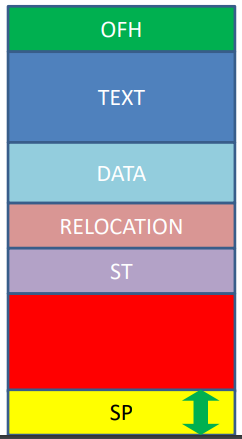
\includegraphics[width=0.30\linewidth]{disposizione file oggetto.png}
    \caption{\textbf{Disposizione dei file oggetto in memoria}}
    \label{fig:enter-label}
\end{figure}
\newpage
\subsection{Collegatore (Linker)}
Quando un programma simbolico è costituito da più moduli contenuti in diversi file sorgenti il processo di traduzione (compilazione e assemblaggio) è ripetuto per ciascun modulo.\par\medskip\noindent 
I \textbf{file oggetto} (object) risultanti devono essere \textbf{collegati} (linked) opportunamente tra di loro all’interno di unico file eseguibile, che solo allora può essere caricato in memoria.\par\medskip\noindent
Per ogni modulo tradotto separatamente l’indirizzo iniziale è lo stesso: è compito del linker modificare gli indirizzi di ciascun modulo in modo che non ci siano sovrapposizioni.
La traslazione dell’indirizzo di ogni istruzione in ciascun modulo permette di unire tutti i moduli ma non è sufficiente, infatti: è necessario traslare in maniera consistente anche tutti gli indirizzi (assoluti) che compaiono come operandi.\par\medskip\noindent
Per ogni riferimento da parte di un modulo a un indirizzo di un altro modulo è necessario calcolare coerentemente l’\textbf{indirizzo esterno} (riferimento esterno o external reference). Esempi in questo senso sono le \textbf{variabili globali}. (che devono essere viste da tutti i moduli) e le chiamate tra procedura appartenenti a moduli diversi.\par\medskip\noindent
Per questo, il linker costruisce una tabella dei moduli grazie alla quale è possibile procedere alla rilocazione e al calcolo dei riferimenti esterni a ciascun modulo.\par\medskip\noindent 
\textbf{ Infine il linker produce un file eseguibile che di norma ha la stessa struttura di un file oggetto, ma non contiene riferimenti non risolti.}\par\medskip\noindent 
\subsection{Caricatore}
Una volta che il file eseguibile è memorizzato sul supporto di massa (generalmente il disco magnetico), il caricatore, o loader, (un programma afferente al sistema operativo) può caricarlo in memoria per l’esecuzione e quindi effettuare:
\begin{enumerate}
    \item la lettura dell’intestazione del file eseguibile per determinare la dimensione dei segmenti testo (istruzioni) e dati.
    \item la creazione un nuovo spazio di indirizzamento, grande a sufficienza per contenere istruzioni, dati e stack.
    \item la copia delle istruzioni e dei dati dal file oggetto al nuovo spazio di indirizzamento.
    \item la copia sullo stack degli eventuali argomenti del programma.
    \item l’inizializzazione dei registri della CPU.
    \item  l’inizio dell’esecuzione a partire da una direttiva di inizio che copia gli argomenti del programma dallo stack agli opportuni registri e che chiama la funzione main() o la direttiva di inizio (BEGIN); fino ad una direttiva di terminazione (END).
\end{enumerate}

\subsection{\textbf{Interprete}}
Un interprete non svolge le operazioni di compilazione e di assemblaggio, ma traduce le istruzioni in linguaggio macchina (memorizzando su file il codice oggetto per essere eseguito dal processore) effettuando solamente una analisi sintattica prima della traslitterazione.\par\medskip\noindent
L’uso di un interprete comporta una minore efficienza durante l’esecuzione del programma (run-time); un programma interpretato, in esecuzione, richiede più memoria ed è meno veloce, a causa dell'overhead (maggior numero di operazioni da compiere) introdotto dall'interprete stesso.\par\medskip\noindent
Durante l'esecuzione, l'interprete deve infatti analizzare le istruzioni a partire dal livello sintattico, identificare le azioni da eseguire (eventualmente trasformando i nomi simbolici delle variabili coinvolte nei corrispondenti indirizzi di memoria), ed eseguirle; mentre le istruzioni del codice compilato, già in linguaggio macchina, sono caricate e istantaneamente eseguite dal processore.\par\medskip\noindent
L'uso di un interprete consente all'utente di agire sul programma in esecuzione sospendendolo, ispezionando o modificando i contenuti delle sue variabili, e così via, in modo spesso più flessibile e potente di quanto si possa ottenere, per il codice compilato.
\newpage
\section{Architettura MIPS}
Il \textbf{MIPS} (\textit{Microprocessor without interlocked pipeline stages}) è un’architettura informatica per microprocessori RISC sviluppata da MIPS Computer Systems Inc (oggi MIPS Technologies Inc).\par\medskip\noindent
Progetto sviluppato nel 1981 da John L. Hennessy dell’Università di Stanford.\par\medskip\noindent 
Suddivisione della \textbf{Memoria Centrale in due parti fisiche} (Memoria Istruzioni e Memoria Dati) per garantire l'esecuzione di una istruzione in un solo ciclo di clock. \par\medskip\noindent 
Realizzazione di una architettura di tipo RISC e in grado di realizzare la tecnica della canalizzazione (pipeline).\par\medskip\noindent
\textbf{Istruzioni RISC} sono caratterizzate da: \textbf{semplicità} (nei primi modelli le moltiplicazioni e le divisioni tra interi furono realizzate con somme e sottrazioni successive) e \textbf{pochi modi di indirizzamento} (per lo più elementari come LOAD e STORE) per garantire l’esecuzione di ciascuna istruzione in un solo ciclo di clock. \par\medskip\noindent
L’esecuzione in un solo ciclo di clock di una istruzione, la suddivisione delle varie unità funzionali e la loro sincronizzazione (ottenuta con l'interposizione di blocchi, un insieme di registri e linee di controllo che sorvegliano il completamento delle varie istruzioni) consentono un \textbf{pipeline regolare} e quindi una \textbf{prestazione della macchina più efficiente} in termine di quantità di calcoli in unità temporale.\par\medskip\noindent
Nel 1984 Hennessy fonda la MIPS Computer Systems.\par\medskip\noindent 
Nel 1985 la società presenta il \textbf{processore R2000} con \textbf{lunghezza della parola a 32bit} nel 1988 è commercializzato il modello R3000 (riduzione della dimensione e del numero dei transistori; frequenza: 20Mhz, 33mhz a 35Mhz). Entrambi i processori sono impiegati come CPU delle workstation della società Silicon Graphics.
Nel 1991 MIPS presenta \textbf{R4000}, il \textbf{suo primo processore a 64 bit}. Acquisizione della società da parte di Silicon Graphics (MIPS Technologies).\par\medskip\noindent
Agli inizi degli anni Novanta, MIPS Tencologies invade il mercato dei microprocessori grazie al basso prezzo e le ottime prestazioni di calcolo offerte dalla canalizzazione.\par\medskip\noindent 
Nel 1997 il MIPS supera il numero di processori venduti da Motorola (uno dei leader del mercato mondiale).\par\medskip\noindent
Nel 1999 MIPS annuncia la possibilità di acquistare la licenza per due processori base: \textbf{MIPS32} a 32 bit e \textbf{MIPS64} a 64 bit.\par\medskip\noindent
Nascita della SandCraft e sviluppo del processore R7100 (eseguiva istruzioni fuori ordine).\par\medskip\noindent 
Creazione della SiByte e produzione del modello SB-1250, uno dei primi processori systems-on-a-chip (SOC) ad alte prestazioni basato su architettura MIPS.\par\medskip\noindent
Fondazione di Alchemy Semiconductor (in seguito acquisita da AMD), che produce il processore di tipo SOC dal nome Au-1000 che necessita di un basso consumo energetico.\par\medskip\noindent
Nella prima metà del XXII secolo l’architettura MIPS trova grossa diffusione nell’ambito dei sistemi embedded, dei device di Windows CE e nei router di Cisco e anche nelle console Nintendo 64, Sony PlayStation, PlayStation 2 e PlayStation Portable.\par\medskip\noindent 
\subsection{Elementi Essenziali}
\begin{figure}[h]
\centering
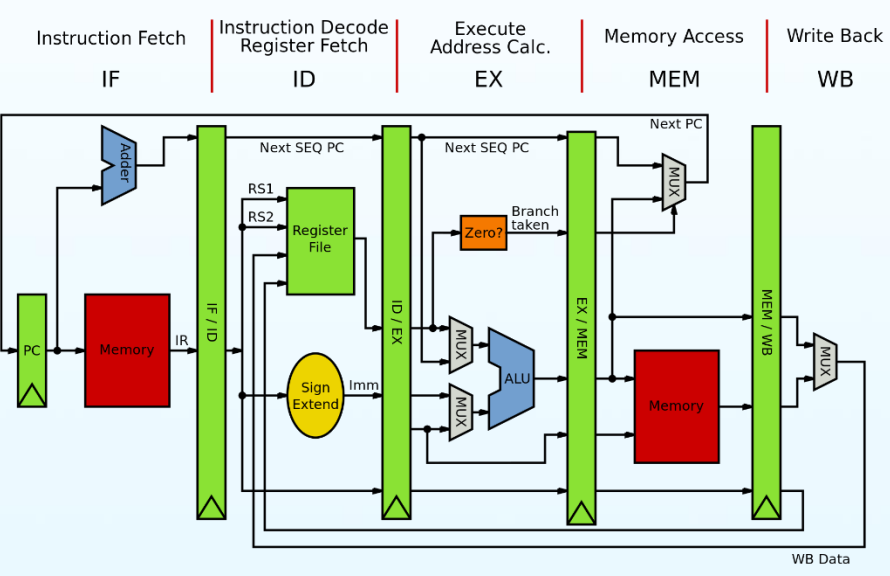
\includegraphics[width=0.75\linewidth]{schema mips.png}
\caption{\textbf{Componenti schema MIPS}}
\label{fig:enter-label}
\end{figure}
\vspace{\baselineskip}
\subsection{I registri}
I \textbf{registri} sono locazioni di memoria in cui ospitare temporaneamente degli operandi/indirizzi/istruzioni.\par\medskip\noindent
\textbf{REGISTRI TEMPORANEI NON PRESERVANTI}: si azzerano dopo un salto a sub-routine.
\begin{lstlisting}
$t0 $t1 $t2 $t3 $t4 $t5 $t6 $t7 $t8 $t9
\end{lstlisting}
\vspace{\baselineskip}
\textbf{REGISTRI TEMPORANEI PRESERVANTI}: mantengono sempre i valori.
\begin{lstlisting}
$s0 $s1 $s2 $s3 $s4 $s5 $s6 $s7 $s8 $s9
\end{lstlisting}
\newpage
\noindent \textbf{REGISTRI TEMPORANEI PER LE SUB ROUTINE:}
\begin{lstlisting}
$a0 $a1 $a2 $a3  #Parametri di ingresso della sub-routine
$v0 $v1          #Risultati della sub-routine
\end{lstlisting}
\vspace{\baselineskip}
\textbf{REGISTRI PER I NUMERI REALI} (NUMERI IN VIRGOLA MOBILE, floating point)
\begin{lstlisting}
$fp0 -------------------------- $fp31
\end{lstlisting}
\vspace{\baselineskip}
\subsection{ALU}
La \textbf{ALU} è il modulo nel quale è presente la circuiteria utile per svolgere operazioni logiche – aritmetiche (adder, shifter, comparator…).\par\medskip\noindent
Il \textbf{MIPS} è dotato di un coprocessore matematico, visto come una unità di I/O con un set di istruzioni specifico, utile per svolgere operazioni aritmetiche con operandi in virgola mobile (espressi in singola e doppia precisione). Questa caratteristica è presente anche nel \textbf{simulatore MARS}.\par\medskip\noindent
\begin{figure}[h]
\centering
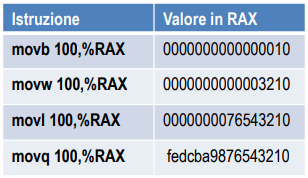
\includegraphics[width=0.75\linewidth]{image.png}
\caption{Componenti – ALU e Coprocessore Matematico}
\label{fig:enter-label}
\end{figure}
\newpage
\subsection{Coprocessore Matematico}
Il \textbf{coprocessore matematico} opera su numeri reali - rappresentati in Virgola Mobile Singola Precisione e Doppia Precisione - siti in memoria oppure numeri interi derivati dal calcolo dell’ALU e stipati nei registri (o in memoria) previa conversione nel formato IEEE754 mediante apposite funzioni di trasformazione.\par\medskip\noindent
\begin{figure}[h]
\centering
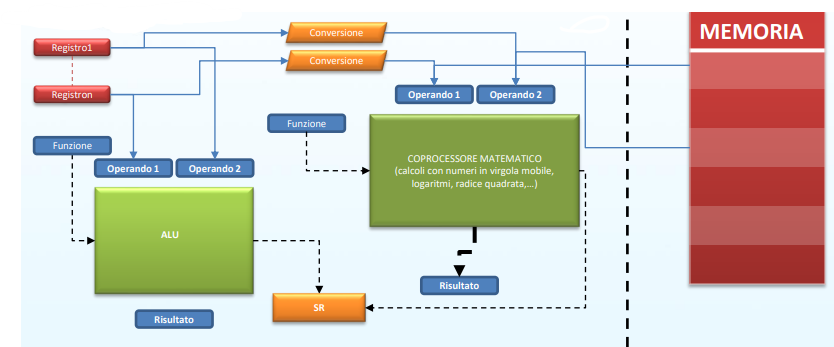
\includegraphics[width=1\linewidth]{coprocessore.png}
\caption{\textbf{Coprocessore}}
\label{fig:enter-label}
\end{figure}
\subsection{La memoria}
Il MIPS ha \textbf{due memorie distinte}:
\begin{itemize}
\item \textbf{Memoria Istruzioni}: area nella quale sono stipate le istruzioni afferenti ad un programma, e una serie di informazioni ausiliarie (stack, kernel S.O., …) 
\item \textbf{Memoria Dati}: area nella quale sono stipati i dati utilizzati dal programma.\par\medskip\noindent
\end{itemize}
\subsection{Componenti – I/O}
I \textbf{dispositivi di Ingresso e di Uscita} (Input Output device o I/O device) permettono l’interazione con il mondo esterno. Il MIPS interagisce con molte periferiche (scheda audio, video, terminale video, tastiera).\par\medskip\noindent
Finestra di input per l’immissione dei dati da tastiera 
\begin{lstlisting}
li $v0,5      #servizio di lettura di un intero da tastiera
syscall       #chiamata di sistema
move $t0,$v0  #spostamento del valore letto da tastiera
          #residente in $v0 dopo la syscall
\end{lstlisting}
\newpage
\noindent Finestra di output (mostrata dal simulatore) per la visualizzazione dei risultati.
\begin{lstlisting}
move $a0,$t0   #spostamento del valore intero da stampare da $t0 a $a0
li $v0,1       #servizio di stampa di un intero
syscall        #chiamata di sistema
\end{lstlisting}
\vspace{\baselineskip}
\textbf{Esempio 1} (Interazione con i dispositivi di I/O)
\begin{lstlisting}
.text
.globl main
main:
li $v0,5       #servizio di lettura di un intero da tastiera
syscall        #chiamata di sistema
move $t0,$v0   #spostamento del valore letto da tastiera residente 
               in $v0 dopo la syscall
add $t0,$t0,1  #calcolo del valore successivo
move $a0,$t0   #spostamento del valore da stampare da $t0 a $a0
li $v0,1       #servizio di stampa di un intero
syscall        #chiamata di sistemali
$v0,10
syscall
\end{lstlisting}
\vspace{\baselineskip}
\section{Linguaggi di Programmazione}
Un \textbf{linguaggio di programmazione} è un linguaggio formale che specifica un insieme di istruzioni le quali sono usate per eseguire un algoritmo e produrre un risultato.\par\medskip\noindent
Il primo linguaggio di programmazione della storia è il «linguaggio meccanico» adoperato da Ada Byron \textbf{Lovelace} per la programmazione della macchina di Charles Babbage nel 1842, si trattava di una sorta di linguaggio assemblativo in grado di mascherare istruzioni e i comandi binari utili per attivare la macchina (studi analoghi furono condotti precedentemente da Luigi Federico Menabrea).\par\medskip\noindent
I sistemi di calcolo automatico degli anni Venti e Trenta del XX secolo impiegano il \textbf{linguaggio macchina}, in cui è fondamentale la conoscenza dell'architettura della macchina.\par\medskip\noindent 
Il \textbf{linguaggio macchina} è basato su codici (stringhe binarie), con il significato di istruzioni, operandi e indirizzi ed è utilizzato dall’elaboratore per eseguire programmi.\par\medskip\noindent
Dopo la seconda Guerra Mondiale con lo sviluppo dell'informatica si usa il \textbf{linguaggio assemblativo} (assembly) il quale introduce una rappresentazione simbolica del linguaggio macchina.\par\medskip\noindent
Il \textbf{linguaggio assemblativo} prevede una rappresentazione dei codici binari del linguaggio macchina con dei mnemonici: si utilizzano simboli invece di stringhe binarie per rappresentare istruzioni, operandi, indirizzi e registri.\par\medskip\noindent
\newpage
Una \textbf{istruzione} di un generico linguaggio assemblativo è strutturata in campi:
\begin{itemize}
\item \textbf{INDIRIZZO}: l’indirizzo dove è memorizzata l’istruzione
\item \textbf{ETICHETTA}: un identificatore che individua la locazione di memoria corrente (opzionale)
\item \textbf{ISTRUZIONE}: l’istruzione da eseguire che prevede \textbf{OPCODE}(è un codice che identifica l’istruzione da eseguire) e  \textbf{MODO DI INDIRIZZAMENTO}(è un codice che esplicita il modo in cui devono essere reperiti i valori con cui si deve operare).
\item COMMENTO
\end{itemize}
\textbf{Struttura di una istruzione, esempio:}
\begin{lstlisting}
INDIRIZZO ETICHETTA ISTRUZIONE          COMMENTO
100:                li $t0,0            # inserimento valore 0 in $t0
104:                li $t1,1            # inserimento valore 1 in $t1
108:                li $t6,10           # inserimento valore 10 in $t6
112:      salto:
116:                add $t0,$t0,$t1     # somma di $t1+$t0 in $t1
120:                bne $t0,$t6,salto   # se il contenuto di $t0 e
                                        # diverso dal contenuto di $t6 
                                        allora vai a salto
\end{lstlisting}
\vspace{\baselineskip}
In seguito, si cercò di astrarre la conoscenza della architettura della macchina mediante i \textbf{linguaggi ad alto livello}.\par\medskip\noindent 
I primi a raggiungere una certa popolarità furono il Fortran (1957); il BASIC (1964); il Lisp (1959); l'ALGOL (1960); Simula (1967); il Pascal (1970) e il C (1972). \par\medskip\noindent 
Nel 1983 vede la luce Smalltalk, il primo linguaggio realmente e completamente ad \textbf{oggetti}; poi lo Eiffel (1986), il C++ (1986) e Java (1995).\par\medskip\noindent
I linguaggi di programmazione ad alto livello sono caratterizzati dalla presenza di astrazioni che permettono al programmatore di non specificare certi tipi di dettagli implementativi della macchina.\par\medskip\noindent
\subsection{Progettazione di un programma}
Come gia detto in precedenza, l’esecuzione di un programma è il punto di arrivo di una sequenza di azioni che nella maggior parte dei casi iniziano con la scrittura di un programma in un linguaggio simbolico di alto livello.\par\medskip\noindent
Le azioni principali che compongono tale sequenza nel caso in cui si parte da un linguaggio ad alto livello sono quelle che vedono in gioco il compilatore, l’assemblatore il collegatore.\par\medskip\noindent
Alcune di queste azioni sono unificate per ridurre il tempo di traduzione, ma concettualmente tutti i programmi passano sempre attraverso le fasi mostrate.\par\medskip\noindent
Nel simulatore MARS la memoria è suddivisa in segmenti. \par\medskip\noindent Ogni segmento è utilizzato per un particolare scopo. \textbf{Segmenti principali}:
\begin{itemize}
\item  \textbf{Text}: Contiene il codice dei programma 
\item \textbf{Data}: Contiene i dati “globali” dei programmi
\item \textbf{Stack}: Contiene i dati “locali” delle funzioni
\end{itemize}
\begin{figure}[h]
\centering
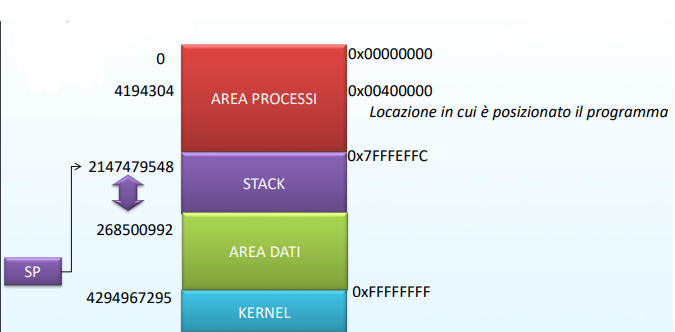
\includegraphics[width=0.60\linewidth]{mars.png}
\caption{\textbf{Memoria del simulatore MARS}}
\label{fig:enter-label}
\end{figure}
\begin{figure}[h]
\centering
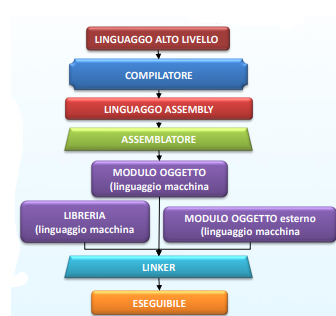
\includegraphics[width=0.50\linewidth]{introduzione.png}
\caption{\textbf{Come funziona un programma}}
\label{fig:enter-label}
\end{figure}
\newpage
\section{Simulatore MARS}
MARS è un ambiente di sviluppo interattivo (\textbf{IDE}) leggero per la programmazione in linguaggio assembly MIPS, destinato all'uso a livello didattico.\par\medskip\noindent 
MARS è un simulatore che esegue programmi per le architetture MIPS - R2000/R3000.\par\medskip\noindent 
Può leggere ed assemblare programmi scritti in linguaggio assembly MIPS. Esso contiene un debugger per poter analizzare il funzionamento dei programmi.\par\medskip\noindent
Compito principale di un linguaggio assemblativo è quello di consentire una programmazione immediata.\par\medskip\noindent
Un linguaggio assemblativo (tra cui il MARS): 
\begin{itemize}
\item Utilizza di parole mnemoniche per identificare le istruzioni del linguaggio macchina.
\item Aumento del numero di istruzioni disponibili per il programmatore attraverso l’uso di pseudoistruzioni.
\item Possibilità di definire macro (gruppo di istruzioni).
\item Possibilità di definire etichette (al posto di indirizzi).
\item Possibilità di aggiungere commenti
\end{itemize}
\vspace{\baselineskip}
\textbf{VANTAGGI E SVANTAGGI}\par\medskip\noindent
\textbf{Vantaggi:}
\begin{itemize}
\item Realizzare sistemi real time
\item Ottimizzare sezioni critiche dal punto di vista della performance di un programma 
\item Utilizzare istruzioni particolari del processore altrimenti non utilizzate dai compilatori (ad es., istruzioni MMX)
\item Sviluppare il kernel di un sistema operativo, che necessita di istruzioni particolari per gestire la protezione della memoria
\item Eliminare vincoli dettati dall’espressività dei costrutti di un linguaggio ad alto livello 
\item Utilizzare le astrazioni dei linguaggi ad alto livello.\par\medskip\noindent
\end{itemize}
\newpage
\textbf{Svantaggi:}
\begin{itemize}
\item Complesso
\item Specificare tutti i dettagli implementativi
\item Scarsa leggibilità del codice
\item Scarsa gestione del codice 
\item Programmatore è supervisore e super gestore 
\item Scarsa produttività 
\item Non portabilità del codice 
\item Massima efficienza dei compilatori\par\medskip\noindent
\end{itemize}
\subsection{Le direttive}
Le direttive forniscono informazioni addizionali utili all’assemblatore per gestire l’organizzazione del codice. Sono identificatori (etichette che iniziano per un carattere alfabetico e sono seguiti da caratteri alfanumerici e il simbolo \textunderscore) che iniziano con un punto.\par\medskip\noindent
\textbf{Esempi} di direttive per il MARS sono: 
\begin{itemize}
\item \textbf{.text}: indica che le linee successive contengono istruzioni
\item \textbf{.data}: indica che le linee successive contengono dati 
\item \textbf{.end}: indica la fine del programma 
\item \textbf{.global}: indica funzioni, variabili globali (accessibili da diversi moduli) 
\item \textbf{.macro}: definisce una macro (un insieme di istruzioni sono descritte da una etichetta)\par\medskip\noindent 
\end{itemize}
\subsection{Tipi di Dati}
Il MARS gestisce 4 tipi di dati: 
\begin{itemize}
\item interi con lunghezza ad otto bit (byte); a sedici bit (half); e a 32bit (word); 
\item reali in singola precisione a 32bit (float) e in doppia precisione a 64bit (double) 
\item stringhe con terminatore (asciiz) e senza terminatore (ascii) 
\item spazi di memoria allocabili (space)
\end{itemize}
\subsubsection{Direttive – Tipi di dati: definizione}
Definizione dei tipi del MARS:
\begin{itemize}
\item .byte b1 , …, bn Alloca n quantità a 8 bit (byte) successivi in memoria
\item .half h1, …, hn Alloca n quantità a 16 bit (halfword) successive in memoria
\item .word w1, …, wn Alloca n quantità a 32 bit (word) successive in memoria
\item .float f1, …, fn Alloca n valori a singola precisione (floating point) in locazioni successive 
\item .double d1, …, dn Alloca n valori a doppia precisione (double point) in locazioni successive di memoria
\item .asciiz str Alloca la stringa str in memoria, terminata con il valore 0
\item .space n Alloca n byte, senza inizializzazione\par\medskip\noindent 
\end{itemize}
L’impiego degli operandi con diversi tipi avviene come nel seguente esempio:
\begin{lstlisting}
.data
Val8bit: .byte 127
Val16bit: .half 70000
Val32bit: .word 5678
Array32bit : .word 1000202, 52462, 3876865
Stringa: .asciiz "Ciao a tutti"
Vettore10byteliberi: .space 10
\end{lstlisting}
\vspace{\baselineskip}
\subsection{Etichette}
Una \textbf{etichetta} (specificata da un identificatore ovvero una stringa alfanumerica che inizia per un carattere alfabetico) individua un punto del programma in cui si trova, cioè un indirizzo.\par\medskip\noindent
Una etichetta consiste in un identificatore seguito dal simbolo due punti {A, …,Z, a…,z} {A,…Z,a,…,z,0,…,9}* {:} \par\medskip\noindent\textbf{Esempio}: main:, loop:, store:, Size:, Array:, Result:, …\par\medskip\noindent
L’etichetta può avere una visibilità locale o una visibilità globale.\par\medskip\noindent
Le etichette sono locali; l’uso della direttiva .globl rende un’etichetta globale.\par\medskip\noindent
Una etichetta locale può essere referenziata solo dall’interno del file in cui è definita; una etichetta globale può essere referenziata anche da file diversi da quello in cui è definita\par\medskip\noindent
\newpage
\noindent \textbf{Esempio:}
\begin{lstlisting}
.text
.globl main
main:
lw $a0, Size
li $a1, 0
li $a2, 0
li $t2, 4
loop:
mul $t1, $a1, $t2
lw $a3, Array($t1)
add $a2, $a2, $a3
add $a1, $a1, 1
beq $a1, $a0, store
j loop
store:
sw $a2, Result
.end

.data
Array: .word 1, 2, 3, 4, 5
Size: .word 4
Store: .space 4
Result: .word 0
\end{lstlisting}
\vspace{\baselineskip}
Una etichetta individua anche una locazione di memoria nella quale sono stipati gli operandi
\subsection{I registri}
I registri contengono dati o indirizzi e sono suddivisi in:
\begin{itemize}
 \item \textbf{registri generali}: possono essere utilizzati in qualunque istruzione, a scelta del programmatore (sebbene esistano delle convenzioni)
\item \textbf{registri speciali}: hanno istruzioni dedicate per essere utilizzati
Esistono istruzioni speciali per gestire i registri speciali: Istruzioni “Branch” e “Jump” per il PC. Istruzioni mthi, mtlo, mfhi, mflo per LO ed HI.
\end{itemize}
\newpage
\begin{figure}[h]
\centering
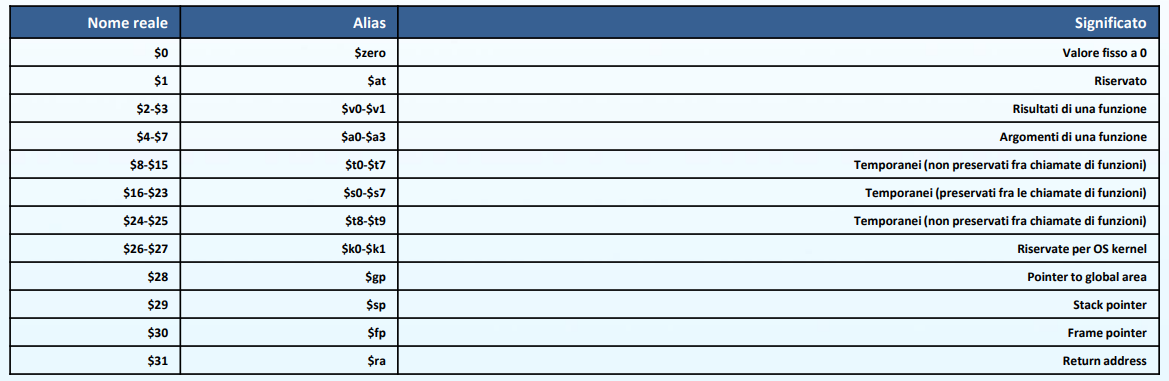
\includegraphics[width=1\linewidth]{registrri-mars.png}
\caption{\textbf{I registri}}
\label{fig:enter-label}
\end{figure}
\vspace{\baselineskip}
I \textbf{registri speciali}: hanno istruzioni dedicate per essere utilizzati
\begin{figure}[h]
\centering
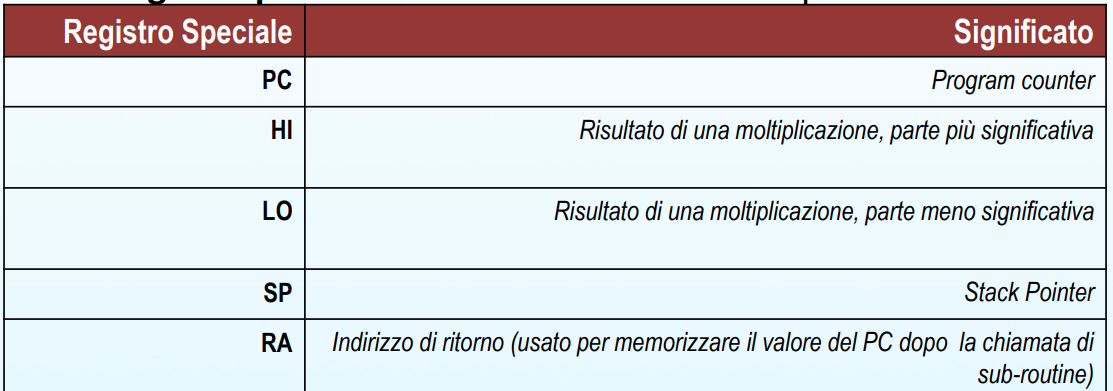
\includegraphics[width=1\linewidth]{registri speciali.png}
\caption{Enter Caption}
\label{fig:enter-label}
\end{figure}
\newpage
\subsection{Istruzioni}
Una \textbf{istruzione} inizia con una parola riservata (keyword) che corrisponde all’OPCODE e continua a seconda della sua sintassi. Esempio: bne reg1, reg2, address (branch if not equal).\par\medskip\noindent
Ad ogni istruzione del linguaggio macchina MIPS corrisponde una istruzione del linguaggio assembly.
\subsubsection{Pseudo- Istruzioni}
Una pseudoistruzione è una istruzione fornita dall’assemblatore ma non direttamente implementata. \par\medskip\noindent Esempio: 
\begin{lstlisting}
blt reg1, reg2, address (branch if less than) 
\end{lstlisting}
\vspace{\baselineskip}
Diventa:
\begin{lstlisting}
slt $at, reg1, reg2 (set less than) bne $at, $zero, address (branch if not equal)
\end{lstlisting}
In pratica una pseudo-istruzione consta di due o più istruzioni.\par\medskip\noindent
\subsubsection{Commenti}
I commenti sono utili per comprendere i singoli passi o l’intero programma (furono un punto di svolta per la programmazione). I commenti non sono inclusi nel modulo oggetto.\par\medskip\noindent
\textbf{Sintassi}: \begin{lstlisting}
#Commento
\end{lstlisting}
\newpage
\section{Architettura funzionale: le istruzioni}
Una \textbf{istruzione} è una stringa binaria che indica all’elaboratore elettronico dei compiti da svolgere.
Una istruzione è suddivisa in sottostringhe denominate campi. La suddivisione in campi individua il formato dell’istruzione.\par\medskip\noindent
Ricordiamo che i campi principali di un'istruzione sono: 
\begin{itemize}
    \item Il \textbf{codice operativo} (o \textit{OPCODE}), che specifica il tipo di operazione da eseguire (addizione, trasferimento dati, …).
    \item L’\textbf{operando}, che indica il dato su cui devono essere effettuate le operazioni indicate dal codice operativo. L’operando può essere un valore numerico (come avviene nell’indirizzamento immediato) o, come spesso accade, si ha un riferimento: cioè, un indirizzo di memoria in cui è immagazzinato un operando (indirizzamento diretto) o una etichetta che specifica un registro.
\end{itemize}
\par\medskip\noindent
Il \textbf{formato a lunghezza fissa} prevede un insieme di istruzioni (instruction set) con una dimensione predefinita (una sottoclasse di questa sono le istruzioni a referenziamento implicito, cioè quelle dotate di solo opcode). \par\medskip\noindent
In alternativa, un set di istruzioni può avere una \textbf{lunghezza variabile}: in relazione al tipo di istruzione cambia la dimensione. Un istruzione a lunghezza variabile di solito ha i bit in eccesso – cioè non rappresentabili nella parola - ospitati nella parola successiva (richiede più accessi in memoria).\par\medskip\noindent
I processori intel X86 hanno un formato a lunghezza variabile. Dopo l’opcode ci sono dei campi che specificano quanti bit appartengono al campo \textbf{MODE}.
\begin{figure}[h]
    \centering
    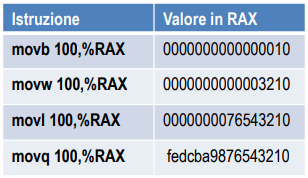
\includegraphics[width=0.5\linewidth]{image.png}
    \label{fig:enter-label}
\end{figure}
\par\medskip\noindent
Il MIPS ha un formato a lunghezza fissa a 32 bit.
Qualora si usi un indirizzamento assoluto (o immediato) in cui il riferimento (o l’operando) richieda più di 16bit l’istruzione è suddivisa in due istruzioni elementari che consentono il riempimento dell’operando/indirizzo in un registro.
\par\medskip\noindent
Le istruzioni sono eseguite quando sono scritte in \textbf{linguaggio macchina} (nei primi elaboratori esisteva solo questo tipo di linguaggio). 
\subsection{Il linguaggio assemblativo}
Il programmatore ricorre ad una rappresentazione simbolica delle istruzioni, utilizzando codici mnemonici che possono essere interpretati in maniera più comoda rispetto alle sequenze binarie: \textbf{istruzioni assembly}.
\par\maketitle\noindent
La sintassi di una istruzione assembly è costituita da:
\begin{itemize}
    \item un indirizzo, dove risiede l’istruzione in memoria (spesso omesso, perché impostato dall’assemblatore).
    \item un'etichetta (opzionale).
    \item un'istruzione composta da: \textbf{codice mnemonico} che descrive l'struzione con pochi caratteri e il \textbf{modo di indirizzamento} cioè i dati su cui deve operare o il luogo dove essi risiedono.
    \item i commenti, indispensabili per la comprensione del codice.
\end{itemize}
\begin{figure}[h]
    \centering
    
\includegraphics[width=0.75\linewidth]{istruszione.png}
    \label{fig:enter-label}
\end{figure}
\par\maketitle\noindent 
Il legame che intercorre tra \textbf{istruzione macchina} e \textbf{istruzione assembly} è di uno a uno, nel senso che ad ogni istruzione macchina corrisponde una ed una sola istruzione assembly. Per comodità molti linguaggi assembly utilizzano delle pseudoistruzioni ovvero delle istruzioni che sono composte da una o più istruzione assembly elementare.
\subsubsection{Le macro}
Un linguaggio assembly consente di definire delle \textbf{macro}: una macro sostituisce una serie di istruzioni. Ogni volta che si richiama la macro l’assemblatore riscrive le istruzioni definite nella macro.\par\medskip\noindent
Prima della fase di assemblaggio a doppia passata si effettua un pre-assemblaggio dove accadono queste operazioni: si risolvono le macro, le pseudo istruzioni, eventuali file esterni e si inizializzano le direttive.
\subsubsection{Esecuzione istruzioni logiche aritmetiche e codici}
Ad ogni tempo, dettato dal \textbf{clock}, l’elaboratore esegue una istruzione. Ogni istruzione logico-aritmetica, produce dei bit, definiti \textbf{flags} (codici di condizione, o condition code), che saranno implicitamente memorizzati nel registro di stato (PSW, processor status word, o STATUS register).
I \textbf{Condition Codes} svolgono un ruolo fondamentale per le istruzioni di salto condizionato.
\newpage
I principali flags sono:
\begin{itemize}
    \item \textbf{C - Carry}: Individua il trabocco ed è impostato ad 1 se l’ultima operazione effettuata dall’ALU ha prodotto un riporto (addizione) o un prestito (sottrazione) a sinistra del bit più significato del risultato, 0 altrimenti.
    \item \textbf{N - Negative}: impostato ad 1 se l’ultima operazione effettuata dall’ALU ha prodotto un risultato negativo, 0 altrimenti. Ovvero Negative è una copia del bit più significativo del risultato.
    \item \textbf{Z - Zero}: impostato ad 1 se l’ultima operazione effettuata dall’ALU è nulla, 0 altrimenti.
    \item \textbf{W - Overflow}: impostato ad 1 se l’ultima operazione effettuata dall’ALU ha superato la capacità di rappresentazione data dalla lunghezza della parola, 0 altrimenti.
    \item \textbf{P - Parity}: impostato ad 1 se l’ultima operazione effettuata dall’ALU ha dato un risultato con un numero pari di 1; 0 altrimenti.
\end{itemize}
\begin{figure}[h]
    \centering
    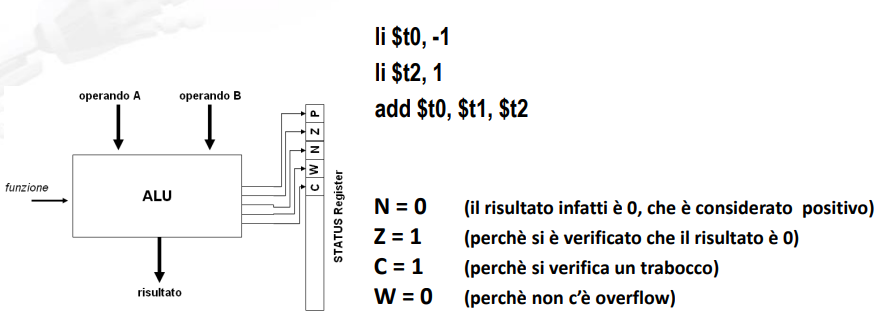
\includegraphics[width=1\linewidth]{flas.png}
    \caption{Codici condizione}
    \label{fig:enter-label}
\end{figure}
\newpage
\subsection{Le classi di Istruzioni}
Possiamo riassumerle in:
\begin{enumerate}
    \item istruzione di spostamento dati
    \item istruzioni logico ed aritmetiche
    \item istruzioni di salto: condizionato, non condizionato, a funzione (o subroutine), trap
    \item  istruzione di controllo macchina
\end{enumerate}
\par\maketitle\noindent 
\subsubsection{ISTRUZIONI DI SPOSTAMENTO}
Le \textbf{istruzioni per lo spostamento} dei dati servono a ricopiare un dato da una sorgente ad una destinazione e cioè da: memoria a registro, registro a memoria, registro a registro, memoria a memoria.\par\medskip\noindent
Le istruzioni di spostamento possono interessare la CPU e la Memoria (LOAD, STORE, PUSH e POP) o solamente i registri nella CPU (MOVE). Il contenuto della destinazione non si modifica rispetto alla sorgente.
\begin{figure}[h]
    \centering
    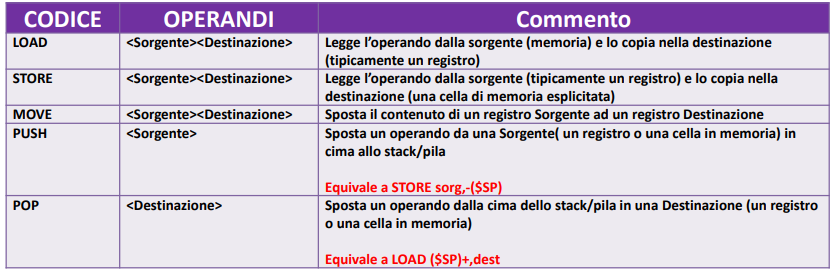
\includegraphics[width=1\linewidth]{istruzioni di spostamento.png}
\end{figure}
\newpage
\subsubsection{ISTRUZIONI LOGICHE-ARITMETICHE}
\textbf{Istruzioni aritmetiche}:  consentono di effettuare le operazioni su numeri interi binari rappresentati in complemento a due (in alcuni casi le ALU possono svolgere operazioni anche con numeri in virgola mobile, ma spesso queste operazioni sono demandate ad una unità di calcolo – il coprocessore matematico - che è visto come un dispositivo di I/O). Le funzioni di base offerte dalla ALU sono il complemento, la comparazione e l’addizione; operazioni come la moltiplicazione o la divisione e la sottrazione possono essere ricavati sfruttando algoritmi che impiegano le operazioni elementari sopra citate. Le istruzioni aritmetiche sono eseguite dall’ALU la quale produce due linee di uscita: \textbf{il risultato dell’operazione} e un vettore di bit, o \textbf{flags} (condition code), che viene implicitamente caricato nello Status Register.
\begin{figure}[h]
    \centering
    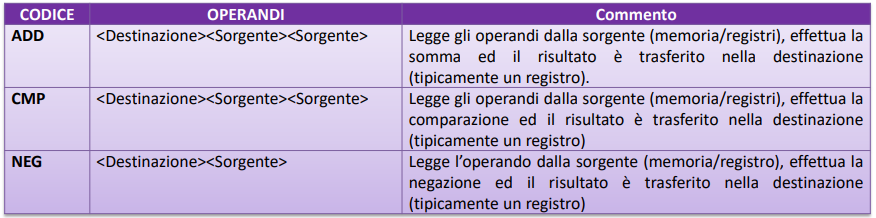
\includegraphics[width=1\linewidth]{operazioni logico aritmetiche.png}
\end{figure}
\par\maketitle\noindent \\ 
\textbf{Istruzioni logiche}: Le operazioni logiche permettono l’esecuzione delle più importanti operazioni definite nell’algebra booleana su stringhe binarie. Come per le operazioni aritmetiche, anche in questo caso, le operazioni avvengono per tutti i bit in posizione corrispondente. La sintassi è simile alle istruzioni aritmetiche e l’operando sorgente può essere in una locazione di memoria, in un registro, o un dato costante (residente dopo l’istruzione); mentre l’operando destinazione è di solito un registro. Anche in questo caso i passi elementari che costituiscono la fase di decodifica ed esecuzione sono analoghi per tutte le istruzioni. Le istruzioni logiche permettono di modificare alcuni bit di un registro, di esaminare il loro valore o di settarli tutti a 0 o 1.
\begin{figure}[h]
    \centering
    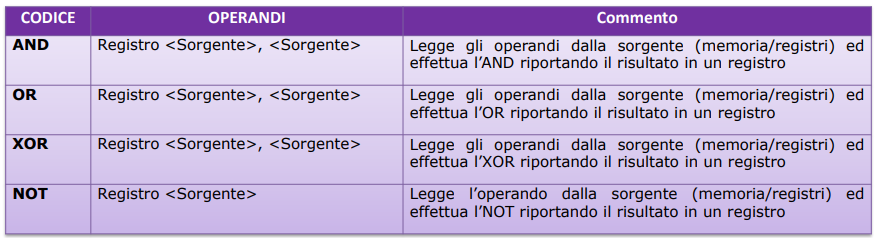
\includegraphics[width=1\linewidth]{operazioni logiche.png}
\end{figure}
\newpage
\noindent \textbf{Le istruzioni di rotazione e shift}: operano su un solo dato posto in un registro. Queste istruzioni cambiano l’ordine dei bit nel registro ed hanno un significato: 
\begin{itemize}
    \item \textbf{logico}: per effettuare lo scorrimento dei bit del registro nella direzione e nel numero di posizioni specificati. Il bit C (carry o trabocco) dello Status Register riceve l’ultimo bit che fuoriesce dal registro; 
    \item \textbf{aritmetico}: è opportuno ricordare che uno shift a destra equivale a dividere l’operando per 2 k (con k il numero di posizioni scorse), mentre uno scorrimento verso sinistra equivale a moltiplicare l’operando per 2k (con k il numero di posizioni scorse)
\end{itemize}
\begin{figure}[h]
    \centering
    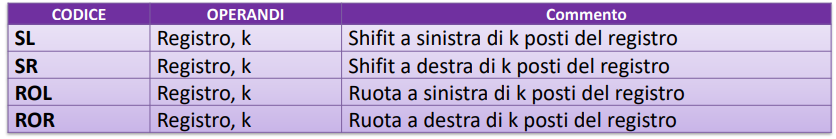
\includegraphics[width=1\linewidth]{shitf e rotazione.png}
\end{figure} 
\par\maketitle\noindent \\ 
\textbf{Istruzioni logico-aritmetiche MIPS}: prevedono un OPECODE comune 000000 che individua la classe e poi una sottodivisione negli ultimi 6 bit che specifica il tipo di funzione.
\begin{figure}[h]
    \centering
    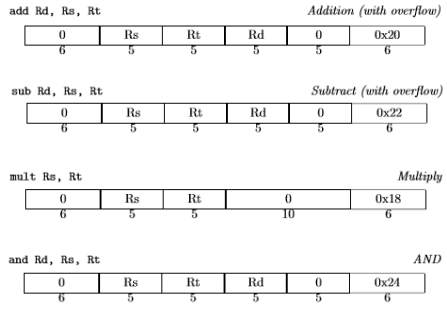
\includegraphics[width=0.75\linewidth]{opecode.png}
    \caption{Enter Caption}
    \label{fig:enter-label}
\end{figure}
\newpage \noindent Esistono inoltre istruzioni, con \textbf{referenziamento implicito}, che consento di operare sui singoli bit del Registro di Stato.
\begin{figure}[h]
    \centering
    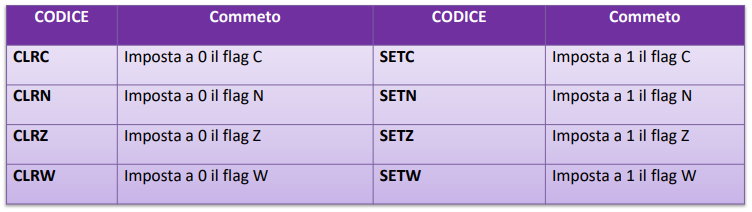
\includegraphics[width=1\linewidth]{Operare sui registri di stato.png}
\end{figure}
\par\maketitle\noindent 
\subsubsection{ISTRUZIONI DI SALTO}
Le istruzioni di salto individuano una classe particolare in quanto non agiscono direttamente sui dati, ma sono utilizzate per modificare l’ordine sequenziale di esecuzione delle istruzioni del programma stesso o uno esterno. \par\medskip\noindent
Le istruzioni di salto si dividono in:
\begin{itemize}
    \item salto all’interno dello stesso programma.\textbf{ Condizionato}: il salto viene eseguito in base ad una certa condizione fissata dal programmatore (Branch).\textbf{ Incondizionato}: il salto viene sempre eseguito (Jump).
    \item salto ad un altro programma: salto a subroutine (salto a sottoprogramma) 
    \item trap (o interruzioni software)
\end{itemize}
\par\maketitle\noindent \\ 
Le \textbf{istruzioni di salto} sono fondamentali perché rompono la sequenzialità offrendo la possibilità di effettuare scelte, cioè, prendere decisioni e perché consentono di eseguire più volte una parte di programma (es.: costrutto IF; ciclo while).
\begin{figure}[h]
    \centering
    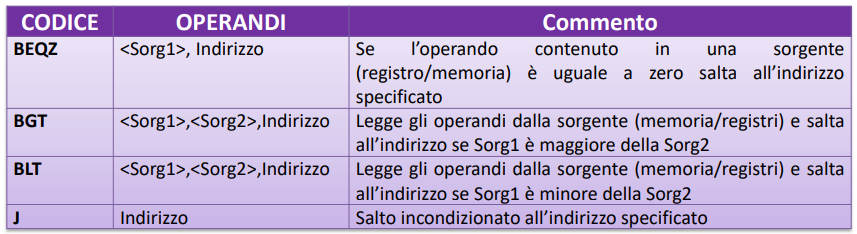
\includegraphics[width=1\linewidth]{salto.png}
\end{figure}
\newpage
\noindent L’\textbf{istruzione di salto a subroutine} (o chiamata a funzione) permette di saltare da un programma (il programma principale) ad un sottoprogramma, di eseguirlo e di tornare alla istruzione immediatamente successiva a quella di chiamata. L’utilizzo di subroutine è utile quando un determinato insieme di istruzioni deve essere eseguito più volte e per avere un codice più chiaro e compatto. Inoltre, le subroutine possono essere realizzate da terzi, essere scambiate e modificate ai propri fini.
\begin{figure}[h]
    \centering
    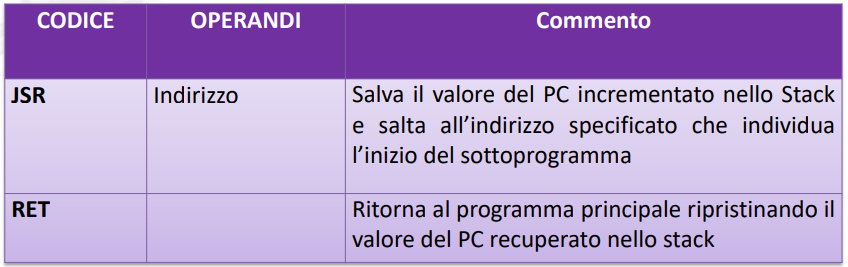
\includegraphics[width=1\linewidth]{subroutine.png}
\end{figure}
\par\maketitle\noindent
Molto spesso però i \textbf{sottoprogrammi possono a loro volta chiamare altri programmi} e così via. Può avverarsi, cioè, un \textbf{annidamento} di subroutine (nested subroutine). In questo caso è fondamentale salvare i diversi indirizzi di ritorno.\par\medskip\noindent
La \textbf{gestione di funzioni ricorsive} o l’annidamento di funzioni avviene grazie all’utilizzo della \textbf{pila} (stack o canasta). Lo stack è una zona di memoria riservata per il passaggio di parametri e la memorizzazione di informazioni gestita nella modalità LIFO (Last in First Out): ovvero l’ultimo elemento immesso nella pila è anche il primo ad uscire.\\
\subsection{Istruzioni I/O}
Per interagire con i dispostivi di I/O si può ricorre ad un set di istruzioni dedicato (IO canonico) o riservare un’area di memoria agli scambi con i dispositivi di I/O ed operare con le istruzioni della macchina (IO programmato).\par\medskip\noindent
Le \textbf{istruzioni di comando} (o istruzioni di controllo macchina) non operano né sui dati né sui registri né interessano il contatore di programma, ma intervengono direttamente sullo stato della CPU. Le istruzioni di comando sono caratteristiche di ogni CPU: il loro numero può variare da poche unità, per macchine semplici, a decine per macchine complesse.
\begin{figure}[h]
    \centering
    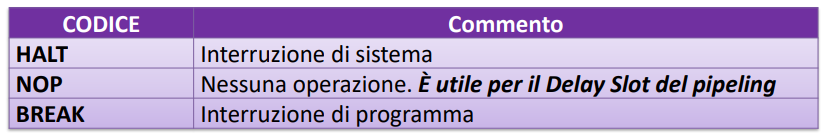
\includegraphics[width=1\linewidth]{input o out.png}
\end{figure}
\subsection{Esempio Pratico}
Realizzazione di un elaboratore che svolga la sola funzione dell’elevamento a potenza di un numero (con esponente\(>\)0) e che utilizza istruzioni a dimensione fissa es.: \(2^3=8\), \(3^3=27\), \(5^2=25\).\par\medskip\noindent
Realizzazione di un elaboratore che svolga la sola funzione dell’elevamento a potenza di un numero (con esponente\(>\)0) e che utilizza istruzioni a dimensione fissa.\\ \\
Possibile implementazione:
\begin{lstlisting}
    LOAD $R0, BASE
    LOAD $R1,ESPONENTE
    LOAD $R2, UNO
    LOAD $R3,MENOUNO
CICLO:
    BEQZ $R1,FINE
    MUL $R2,$R2,$R0
    ADD $R1,$R1,$R3
    JUMP CICLO
FINE:
    STORE $R2, RISULTATO
\end{lstlisting}
\par\medskip\noindent \\
Di cosa si ha bisogno: 
\begin{itemize}
    \item  4 registri enumerati da R0 a R3 
    \item  Una ALU che faccia 4 operazioni: moltiplicazione, somma, salto condizionato al valore zero, salto incondizionato 
    \item  Istruzioni di caricamento e archiviazione dati in memoria 
    \item  Spazio in memoria per archiviare i dati e gli operandi
    \item Numero di istruzioni: 6
    \item Registri: 4 (+ 1 di ausilio alla macchina trasparente al programmatore settato a 0 e non
    modificabile)
\end{itemize}
\par\medskip\noindent \\
\textbf{Domanda}: quanto deve essere lunga la parola per indirizzare almeno 255 locazioni di memoria
(126 per ospitare il programma e 127 per ospitare i dati)?
\end{document}